%!TEX root = ../../Heun_Dale_Haney_A_dynamic_approach_to_input_output_modeling.tex
%%%%%%%%%%%%%%%%%%%%% chapter.tex %%%%%%%%%%%%%%%%%%%%%%%%%%%%%%%%%
%
% sample chapter
%
% Use this file as a template for your own input.
%
%%%%%%%%%%%%%%%%%%%%%%%% Springer-Verlag %%%%%%%%%%%%%%%%%%%%%%%%%%
%\motto{Use the template \emph{chapter.tex} to style the various elements of your chapter content.}
\chapter{Material flows}
% use \chaptermark{}
% to alter or adjust the chapter heading in the running head
\chaptermark{Materials}
% Always give a unique label
\label{chap:materials} 

\abstract*{[NEED TO ADD ABSTRACT HERE]}

%% \abstract{Each chapter should be preceded by an abstract (10--15 lines long) that summarizes the content. The abstract will appear \textit{online} at \url{www.SpringerLink.com} and be available with unrestricted access. This allows unregistered users to read the abstract as a teaser for the complete chapter. As a general rule the abstracts will not appear in the printed version of your book unless it is the style of your particular book or that of the series to which your book belongs.\newline\indent
%% Please use the 'starred' version of the new Springer \texttt{abstract} command for typesetting the text of the online abstracts (cf. source file of this chapter template \texttt{abstract}) and include them with the source files of your manuscript. Use the plain \texttt{abstract} command if the abstract is also to appear in the printed version of the book.}

%% Use the template \emph{chapter.tex} together with the Springer document class SVMono (monograph-type books) or SVMult (edited books) to style the various elements of your chapter content in the Springer layout.

In Chapter~\ref{chap:intro}, we put forward the idea that economies are like organisms. 
This chapter explores
this idea further by observing the interchange of materials \emph{within}
an economy, as well as exchanges of materials between an economy and 
surrounding environment---the biosphere\index{biosphere}. 

% [THE FOLLOWING PARAGRAPH CONNECTS MORE WITH THE METABOLISM METAPHOR,
% NEED TO DECIDE BETWEEN THAT AND THE ONE AFTER OR MAYBE MIX THE TWO]

% Just as a living organism takes
% in food, water and air, so too an
% economy must take in raw materials from its environment. To a large extent,
% the major exchanges of materials between industrial economies and their 
% environment mirror those of an animal. Large inputs of fresh water, hydrocarbons
% and oxygen with the emission of carbon dioxide and polluted water [REF BRANDT]
% dioxide and hydro-carbons These
% materials are then used for a number of different purposes. Some
% become the building blocks from which the physical structures within the 
% economy---buildings, roads, even people---are composed. These materials
% must be extracted from the environment and processed, transported and then
% manufactured into final goods. Such activities require energy resources. In
% an economy primarily dependent on the combustion of fossil fuels, energy conversion
% of energy necessarily requires the presence of oxygen in the atmosphere and
% the emission of carbon dioxide. Many processes also require flows of materials, 
% especially fresh water, that are not directly embodied in the final product.
 

There are many easily observable instances of material flow within an
economy. I look around my office at my computer screen and coffee cup
and myriad other items. I look out my window to the street and building
opposite. All of these goods came originally from natural 
resources\index{natural resources}\index{resources!natural|see{natural resources}}, 
be it paper or petroleum or rock. They were extracted and processed, transported and
transformed requiring yet more materials and energy inputs in the form of
electricity or fuels. 

There are also inumerable material flows caused by an economy that we do not observe.
The extraction of raw materials generates additional overburden---earth that must be
extracted and processed and ultimately discarded without ever entering the economy
proper. Other flows occur around us unseen. The cars outside my window suck in nitrogen
and oxygen (without which the engine would not work) and emit water, carbon dioxide and
other more harmful substances. 

Even services which we tend to think of as non-material, require at least some material
infrastructure. The hairdresser requires scissors (and to a greater or lesser extent 
some hair) with which to work. Even the internet, often lauded as the exemplar of
dematerialization of the economic process, requires a whole host of computer
infrastructure including electricity, data servers, telephone networks and a
computer by which to access it.

In this chapter, we will define a mathematical framework by which to track the flow of
materials within an economy, building from a one-sector economy up to examples of both a
two- and three-sector economy. We will finally apply this framework to the illustrative
example of the US automobile industry that runs through the whole book. First let us
outline the basic methodology.

\section{Methodology}
\label{sec:Materials_Methodology}

% Everyone is familiar with the notion of accounting of material (and even non-material)
% things. In order to be rigorous, the first step requires the definition of what we
% will be counting as well as the place (defined in both time and space) for which we will
% be counting. Engineers often call this a \emph{control volume}. For example, I may wish
% to account the number of apples in my home over a week-long period. In which case,
% I would count the number of apples that enter  and leave my home, as well as any apples
% that are eaten and, just in case I happen to have an apple tree, any apples that grow
% inside my home. Our accounting equation would look something like:

% **** The idea that we are ``counting money'' does not seem exactly 
% right to me. Isn't it that we are accounting for value and energy flows? 
% Later on we will use currency flows to approximate the value flows? BRH ****

This book is about tracking (accounting) flows through the 
economy with a focus on counting materials, energy, and value.
That an entire academic discipline and industry are focused on counting money (``accounting'')
is evidence of its importance in today's economies.
That energy is required to do \emph{anything} is evidence 
of its importance in the economic activity of our daily lives.
And, we believe that the interplay between money and energy
has shaped the past and will continue to influence the future.
In this section, we define rigorous ``counting'' methods that will be applied
to money and energy throughout this book.

[Include somewhere in here the difference between \emph{flows} and \emph{funds}, 
between \emph{efficient cause} and \emph{material cause}. Resources are 
\emph{transformed} into products.]

Everyone counts material (and even non-material) things. 
Rigorous counting requires precise definition of both 
what we will be counting
and the place (defined in both time and space) in which we will be counting. 
Engineers often call the spatial definition a ``control volume.'' 
Another way to think of creating a
control volume is drawing a boundary. 
What gets counted is what passes through the boundary.
For example, we 

**** Do we want to write in the first person? ****
**** Good question. We're using the first person
in most of the chapters, but plural, ``we'', rather than
singular. I've changed the ``I'' to ``we'', but we should
double-check that we're happy with it, as it mixes
plural and singular first person: ``we'' with ``my'' and
``I'' ****

may wish to count (or ``make an accounting of'') 
the stock of apples in my home over the course of a week. 
We draw a spatial boundary (control volume) around my home 
and a temporal boundary ``around'' the week.
We count the apples that enter and leave my home, 
apples that are eaten (consumed),
and, if I own an apple tree, apples that I grow (produce) during a week. 
A rigorous apple accounting equation, in units of apples, is:
\begin{equation}
	\mathrm{\Delta}\mathrm{apples} 
	= \mathrm{apples~in} 
	- \mathrm{apples~out} 
	+ \mathrm{apples~grown} 
	- \mathrm{apples~eaten}.
\end{equation}

\noindent{}More generally, we may say:
\begin{equation}
	\mathrm{Accumulation}
	= \mathrm{Transfers~in} 
	- \mathrm{Transfers~out}
	+ \mathrm{Production}
	- \mathrm{Consumption}.
\end{equation}

Notice that, when discussing apples we use the specific terms ``grown'' and
``eaten'' instead of the more general terms, ``produced'' and ``consumed.''
Later, in Chapter~\ref{chap:value}, when discussing value, we will use the terms
``generated'' and ``destroyed.'' For our purposes, these terms all have the equivalent
meanings and we use them interchangeably.

After accounting for the stock of apples in a week,
we can reframe the questionL ``at what rate does the stock of
apples change?'' That is, we can examine the rate of
change of the apple stock per unit of time relative to the flow of apples 
($\dot{a}$)\nomenclature[ab]{$\dot{a}$}{flow rate of apples [apples/time]}, 
e.g.\ in units of apples per day, 
in which case our accounting equation would become:

\begin{equation} \label{eq:apple_rate_accounting}
	\frac{\mathrm{d}a}{\mathrm{d}t}
	= \dot{a}_{in}
	- \dot{a}_{out}
	+ \dot{a}_{grown}
	- \dot{a}_{eaten}
\end{equation}
\nomenclature[a]{$a$}{stock of apples [apples]}
\nomenclature[t]{$t$}{time [s]}

\noindent{}where the dot above the variable ($\dot{a}$) indicates 
a flow rate per unit time [apples/time] and
the time derivative $\left( \frac{\mathrm{d}a}{\mathrm{d}t} \right)$ 
is the rate of change of the stock of apples per time unit, or more simply,
the accumulation\index{accumulation} rate.
 
% ***** Take a moment to tie apples to mass or material. 
% Clearly note that material is measured kg rather than dollars.
% Note the distinction between material and mass.
% We are doing material accounting in units of mass.
% We will later do material accounting in units of energy.
% Even later, we will do material accouting in units of dollars. ****

Notice, that instead of focusing on apples as our unit of accounting, 
we could track the mass flow, e.g.\ measured in kg/sec, 
of the main chemical elements within the apples. 
From this perspective, although an apple may be consumed,
the elements within the apple---hydrogen, oxygen (coupled together as water
for the overwhelming majority of the mass), 
and carbon (which, bonded with hydrogen as carbohydrates make up most 
of the remaining mass)---will not be consumed. 
The chemical elements will instead be stored within my body, 
leave the house as waste\index{waste}, 
or leave the house via the air as exhaled carbon dioxide (CO$_2$).

%**** Auto industry example here? Perhaps steel? ****

If, instead of a home, we drew a spatial control volume 
around a sector of an economy, 
similar accounting methods can be applied. 
In fact, throughout this book, we will illustrate theoretical concepts with
a running example of the auto industry. 
We choose the auto industry,
because it remains a large portion of most industrialized economies, 
because is very resource intensive,
because it has been used in the literature~\cite{Bullard:1978vd}
to illustrate input-output accounting methods, 
because its links with energy are obvious,
because its health is sensitive to disruptions in energy supplies, and
because it shows evidence of post-industrial decline (shrinking profit margins, etc.).

If we account for steel (in units of kg) in the auto industry, 
we might write an equation like this:

\begin{equation}
	\mathrm{\Delta}\mathrm{steel} 
	= \mathrm{steel~in} 
	- \mathrm{steel~out} 
\end{equation}

Note that the production and consumption terms are zero
since steel is not created or destroyed within the automobile
sector. Tracking the rate flows of steel, 
$\dot{s}$ (in kg/s)\nomenclature[sd]{$\dot{s}$}{steel mass flow rate [kg/s]},
we would write the following equation:

\begin{equation}
	\frac{\mathrm{d}s}{\mathrm{d}t}
	= \dot{s}_{in}
	- \dot{s}_{out}
\end{equation}
\nomenclature[sc]{$s$}{stock of steel [kg]}

Again, the last two terms (steel production and consumption) are not present. 
This is in direct contrast with the apple 
accounting equation outlined in Equation~\ref{eq:apple_rate_accounting}. 
**** Do the previous two sentences make sense?
The equation has only 2 terms. **** 
I have reworded to specify the production and consumption terms. ****
Despite the fact that steel is neither produced nor consumed within the automobile sector, 
there are sectors of the economy that \emph{do} produce steel,
by mixing molten iron with varying amounts of carbon. 
The flow of steel through an economy illustrates that although certain economic
products, e.g.\ steel, may be produced or, in some circumstances, destroyed, the
\emph{mass} of iron, and other chemical elements, is constant,
even as the mass changes form (e.g.\ from iron to steel) 
through many economic processes.\footnote{For the sake of
absolute rigor, we must point out that, in actuality, iron \emph{is} created within
the core of silicon-burning stars. Mass and energy may also be converted in such processes, 
such that only mass-energy is conserved. However, for the purposes of terrestrial
processes, the total mass (in kg) of iron is constant. There are, additionally, some economic
processes, within nuclear reactors, that change the atomic structure of elements
and thus violate the accounting law presented here. Because the mass flows involved
with these nuclear plants is negligible compared with total materials flows, we
shall assume that the law holds.}

% **** Discuss the steel industry. 
% Show how steel is actually formed from other materials.
% Show that \emph{mass} is neither created nor destroyed, 
% but it may change form. ****

Indeed, within the car industry, inputs of steel, glass, plastic, rubber, etc.\ are used
to produce cars, such that cars are created within the automobile industry. 
An accounting equation for cars within the economy
must include terms for production and destruction\footnote{In economic terms,
destruction of physical goods is often called ``depreciation.'' We shall 
explore the importance of and distinctions between 
physical depreciation and economic depreciation 
in Chapters~\ref{chap:embodied_energy}--\ref{chap:implications}.}
of cars.
Again, focussing on mass flows of the chemical elements avoids this necessity, 
because mass is \emph{conserved} in physical processes. 
Conservation of mass is expressed in equations such as the ones above
for apples and steel. 

Another important conservation principle is the conservation of energy.
Similar to the principle of the conservation of mass,
the First Law of Thermodynamics\index{First Law of Thermodynamics},
says that \emph{energy} can neither be created nor destroyed. 
In the discussion that follows, we will make great use 
of the First Law.
If I eat an apple, it is no longer an apple, 
but the materials (i.e.\ chemical elements) and energy contained
within the apple can still be traced via their mass and energy,
even if they change form (apples into compost or 
chemical potential energy to thermal energy).
Thus, the apple accounting equation
(Equation~\ref{eq:apple_rate_accounting}) can include
terms accounting for the production and consumption of apples. 
However, mass and energy accounting equations applied to 
sectors of economies will \emph{not} include terms for the 
production or destruction of mass or energy. 
Rather, any addition of material or energy added \emph{to} the economy
or waste\index{waste} of material or energy \emph{from} the economy
will occur as an interaction between the economy and the biosphere\index{biosphere}.
Chapters~\ref{chap:materials}--\ref{chap:embodied_energy} cover mass and energy
accounting for economies.
Accounting for economic value, in contrast, 
\emph{will} require terms that both create and destroy economic value,
as discussed in Chapter~\ref{chap:value}.


%%%%%%%%%% Materials %%%%%%%%%%
\subsection{Product, resource, short-lived, and capital flows}
%%%%%%%%%%

When applying accounting equations to economic sectors,
we distinguish among four types of
materials flowing into or out of a production sector: 
products ($P$) \nomenclature[P]{$P$}{mass of products [kg]}, 
resources\index{resources} ($R$)\nomenclature[R]{$R$}{mass of resources [kg]},
short-lived goods ($S$)\nomenclature[S]{$S$}{mass of short-lived goods [kg]},
and capital goods\index{capital goods} ($K$)\nomenclature[K]{$K$}{mass of capital goods [kg]}, 
as shown in Figure~\ref{fig:PERKS_materials}.

\begin{figure}[!ht]
\centering{}
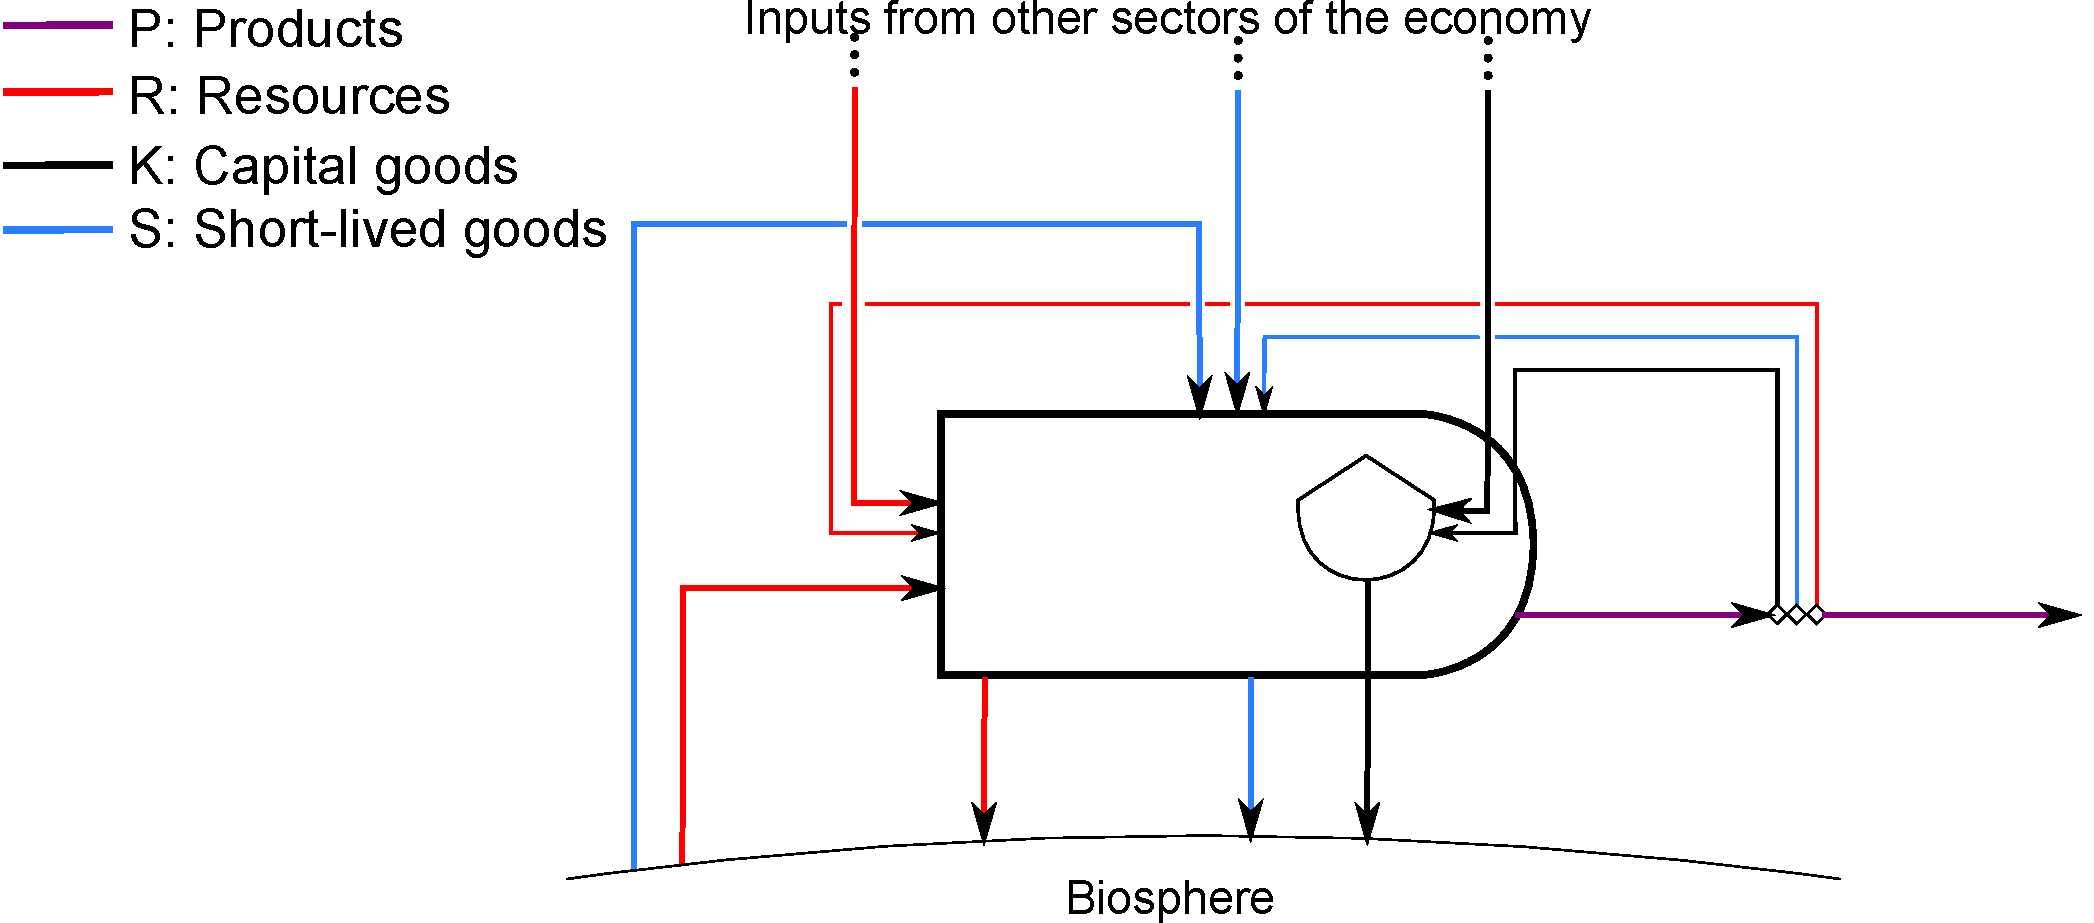
\includegraphics[width=0.8\linewidth]{Part_1/Chapter_Materials/images/PERKS_basic_unit_materials.pdf}
\caption[Material flows into and out of a single sector 
of the economy.]{Material flows into and out of 
a single sector of the economy. 
Resource flows ($\dot{R}$) enter the sector from the left 
and are embodied in products ($\dot{P}$) which leave from the right. 
Some waste\index{waste} resources are leave the sector at the 
bottom and are returned to the biosphere\index{biosphere}.
Short-lived material flows ($\dot{S}$) 
enter the sector from above and leave from below to return to the biosphere. 
Only capital stock ($\dot{K}$) may accumulate within the sector,
depicted by the storage tank.
These also enter the sector from above. 
Depreciated capital leaves the sector from below and is returned to the biosphere.}
\label{fig:PERKS_materials}
\end{figure}

Resource materials ($\dot{R}$)\nomenclature[Rb]{$\dot{R}$}{resource mass flow rate [kg/s]} 
enter the sector on the left 
and comprise those materials that are destined to be \emph{embodied} 
in the goods produced by the sector ($\dot{P}$)\nomenclature[Pb]{$\dot{P}$}{product mass flow rate [kg/s]}, 
except for some proportion that are wasted\index{waste}.
Wastes depart from the bottom of the sector and are
returned to the biosphere\index{biosphere}. 
For example, sheet metal, rubber, and glass
(as well as many other materials) 
enter the automobile sector as resources 
and end up as material parts of the cars that are produced. 
Some fraction of these resources ($\dot{R}$) may not make it into the final product, 
such as trimming scrap from metal parts stamping, 
and may be either recycled internally, 
or wasted\index{waste} to the biosphere\index{biosphere}. 
In this model, resource materials are not accumulated\index{accumulation} within a sector.

Short-lived goods ($\dot{S}$)\nomenclature[Sb]{$\dot{S}$}{short-lived goods mass flow rate [kg/s]}  
include those materials 
that are necessary for the production processes of a sector, 
but are neither accumulated within the sector, 
nor destined to be materially part of the product of the sector. 
They enter the sector from above and leave the sector from
below and return to the biosphere. 
Examples of these short-lived flows include energy resources, such as
the electricity needed to run automobile factories 
% including any contribution from labor, **** contribution from labor seems out of place here --MKH ****
and water used by the sector. 

Many material flows into the sector, such as production equipment,
are necessary for the continued operation of a sector 
but are not counted as short-lived goods, 
because the operation of the sector is dependent 
upon the accumulation\index{accumulation} of these materials within the sector. 
Such flows are counted as capital goods\index{capital goods} 
($\dot{K}$).\nomenclature[Kb]{$\dot{K}$}{capital goods mass flow rate [kg/s]}
Capital flows also enter from above, 
but are stored within the sector (represented by a storage tank) 
and are returned to the biosphere as 
physical capital depreciation\index{physical depreciation} from below.
Examples of these capital flows would be the factory and office buildings or
manufacturing equipment within the automobile industry.
We are here assuming that there is no re-use of capital stock
within other sectors of an economy,
e.g.\ resale of vehicles or other equipment after depreciation,
or recycling of material from capital stock into other goods,
e.g.\ scrap metal. 
The issue of recycling is in greater detail in
Section~\ref{sec:recycling}.

All products ($\dot{P}$) leave the right of the sector. 
A fraction of the $\dot{P}$ flow may be returned to the sector as self-consumption 
counted as resources destined to be embodied in the product ($\dot{R}$), 
short-lived materials ($\dot{S}$), or 
capital goods\index{capital goods} ($\dot{K}$); 
the remainder flows to other sectors within the economy or final demand. 
In this model, energy may be accounted
as either an $\dot{R}$ flow or an $\dot{S}$ flow.
An example of energy as an $\dot{R}$ flow is crude oil converted into
gasoline within a refinery: the resource inflow (crude oil) is
\emph{literally} embodied within the outflowing product (gasoline).
An example of energy as an $\dot{S}$ flow is electricity
used by an automobile factory: the resource inflow (electrons)
is not embodied \emph{literally} in the outflowing product (automobiles).
Similarly, the coal or natural gas flowing into a
power plant is accounted as an $\dot{S}$ flow, 
because the incoming chemical elements (carbon and hydrogen) \emph{do
not} depart the plant as the product.  
(The product of a power plant is electrons that travel through
electricity transmission lines.)

Throughout this book, we illustrate concepts with three example economies, 
with increasing levels of disaggregation. 
Example~A includes a single economic sector (1) and the biosphere (0).
Example~B includes a production sector (2), society (1, which provides final demand),
and the biosphere (0). 
Example~C adds an energy sector (3) to Exammple~B.
We begin with materials accounting for Example~A.


%%%%%%%%%% Materials: Example A %%%%%%%%%%
\section{Example~A: single-sector economy} % chktex 13
\label{sec:A_materials}
%%%%%%%%%%

Our first example looks at the case where all processes within the economy occur within
one sector---Society (1)---which exchanges materials with the biosphere\index{biosphere} (0) as depicted in
Figure~\ref{fig:A_materials}.  We do not distinguish between production and consumption.

\begin{figure}[!ht]
\centering{}
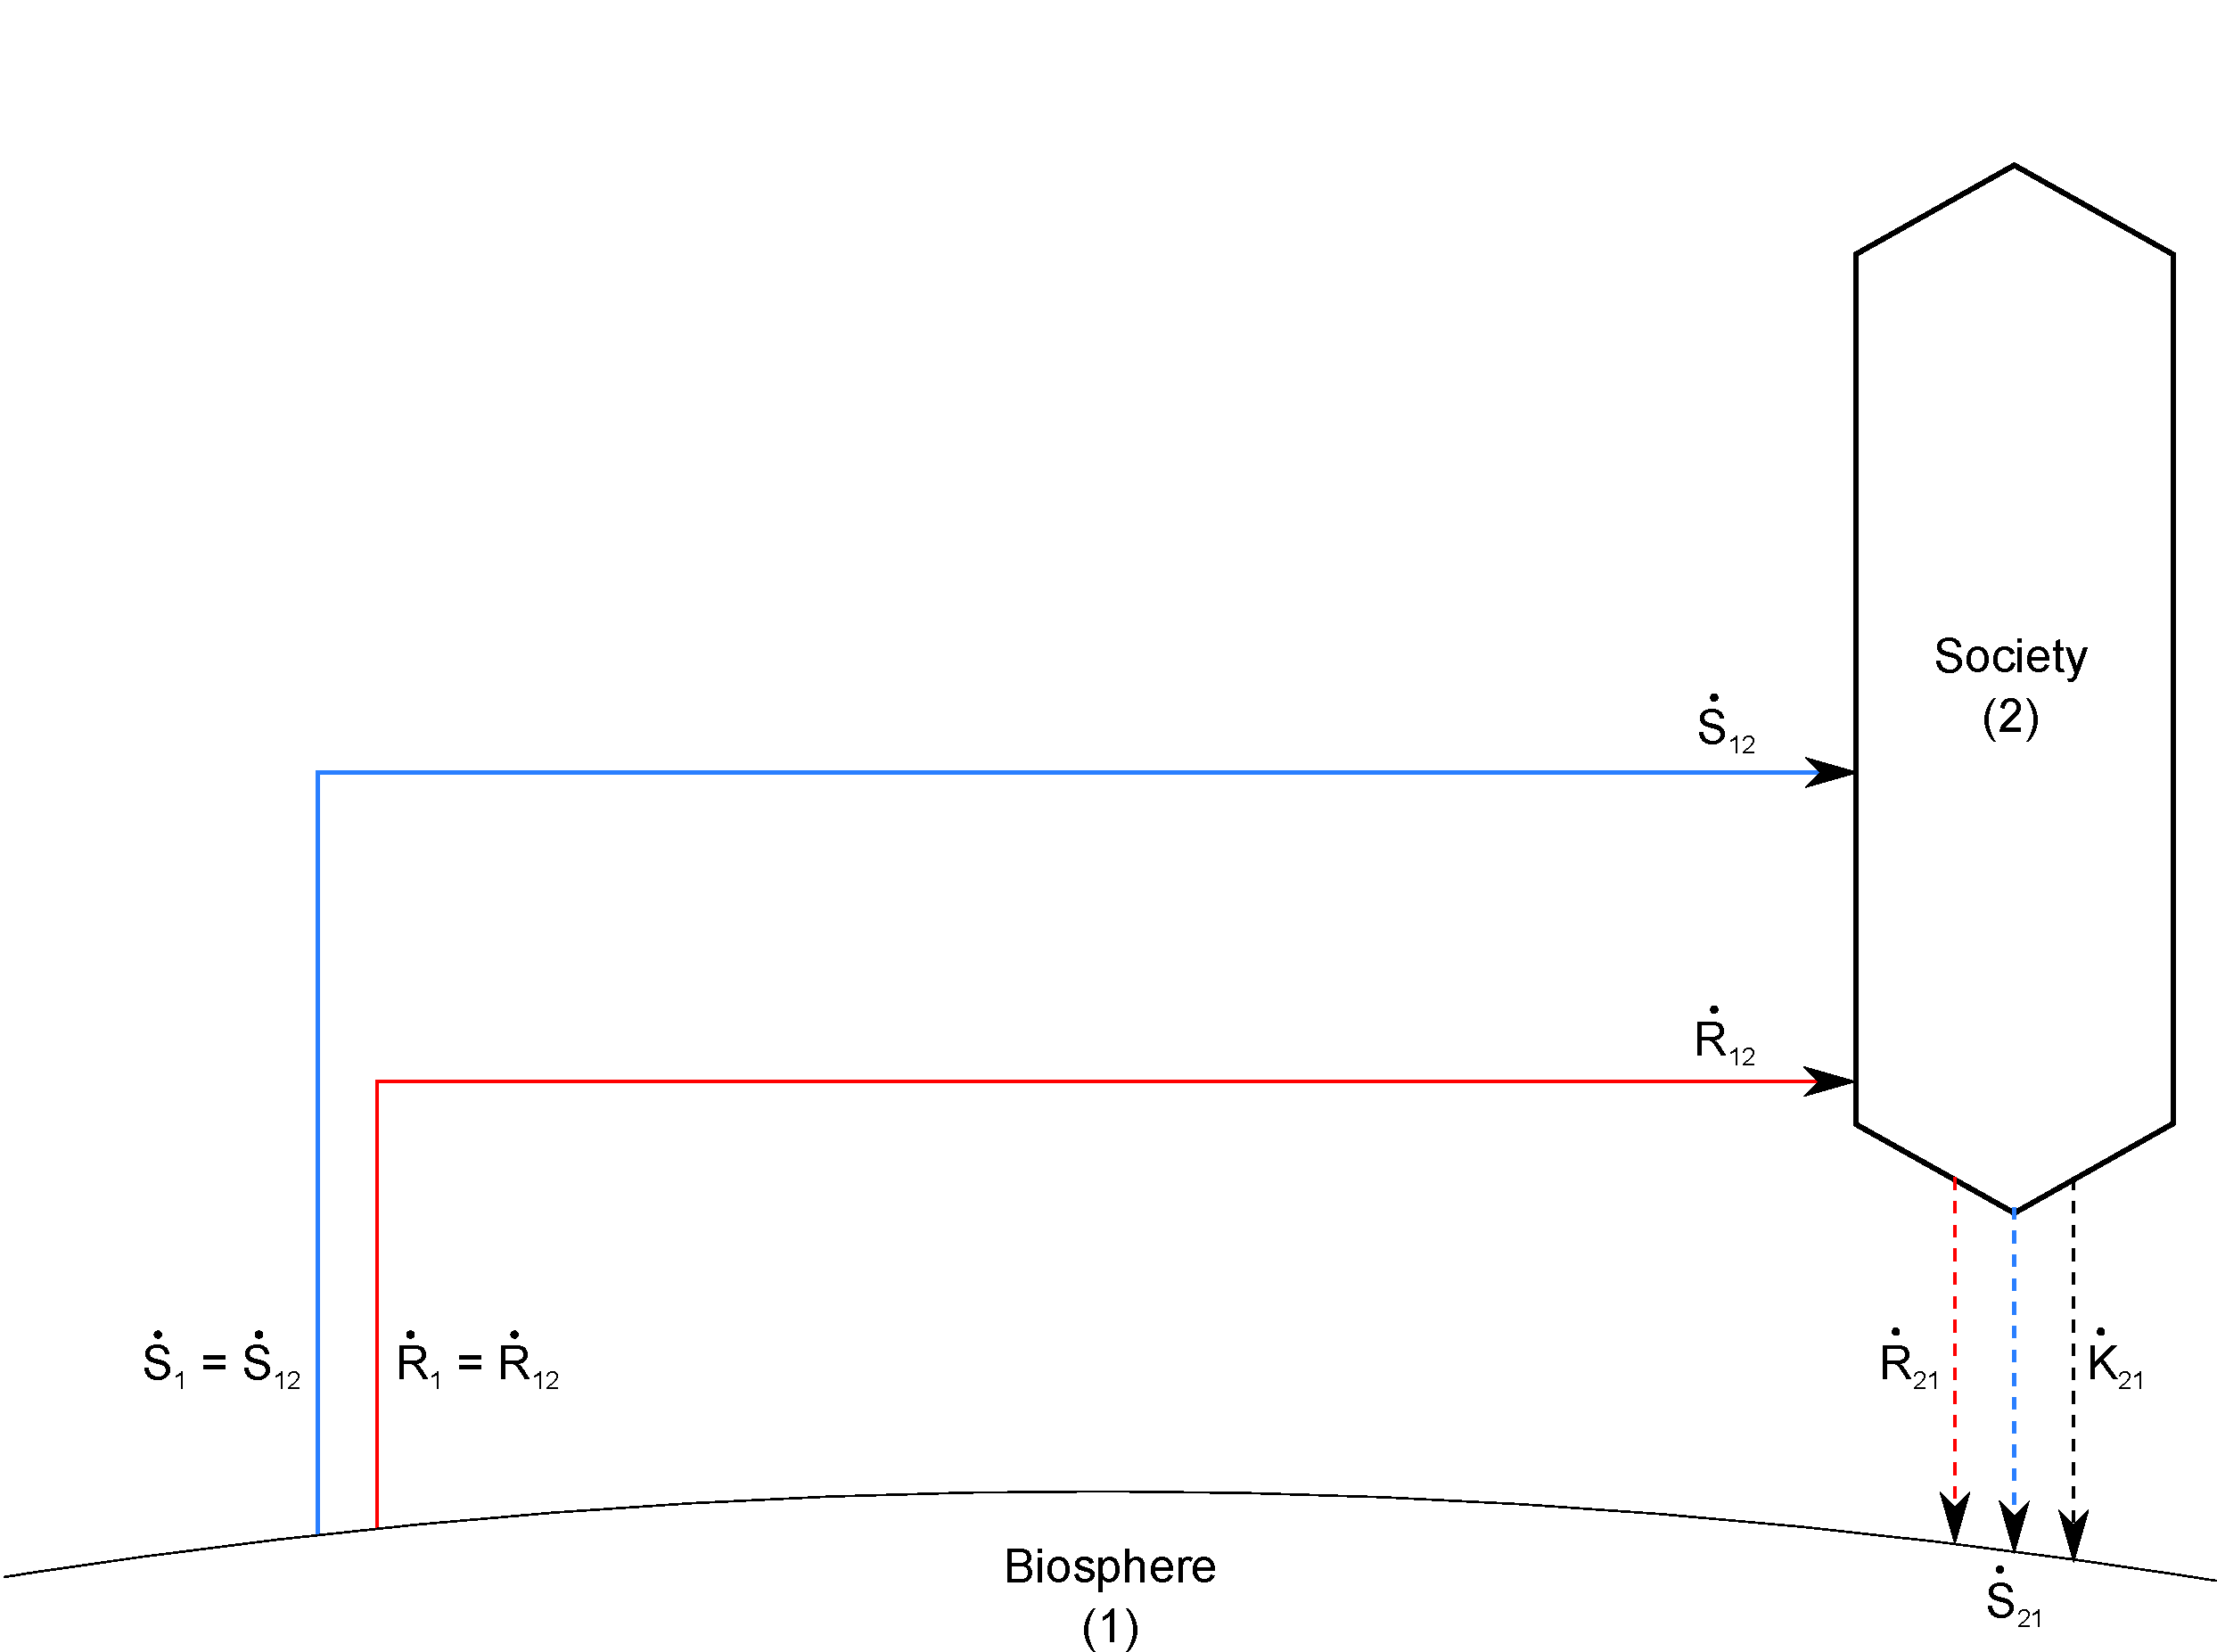
\includegraphics[width=0.8\linewidth]{Part_1/Chapter_Materials/images/1_sector_materials.pdf}
\caption[Flows of materials for a one-sector economy]{Flows of materials 
for a one-sector economy. 
Resources ($\dot{R}_{01}$) and short-lived materials 
($\dot{S}_{01}$) flow into the economy (1) 
from the biosphere\index{biosphere} (0). Waste resources 
($\dot{R}_{10}$) short-lived materials/goods 
($\dot{S}_{10}$) and capital goods\index{capital goods} 
($\dot{K}_{10}$) are returned to the biosphere.}
\label{fig:A_materials}
\end{figure}

Resources, or perhaps more accurately raw materials, 
($\dot{R}_{01}$), such as crude oil or iron ore, 
and short-lived materials ($\dot{S}_{01}$), 
such as oxygen or water that flow \emph{through} economic
processes but are not literally \emph{embodied} within the output, 
flow into the economy (1) from the biosphere\index{biosphere} (0). 
These materials are processed within the economy into products ($\dot{P}_{1}$) 
consisting of resource goods ($\dot{R}_{11}$), 
short-lived goods ($\dot{S}_{11}$) and capital 
goods\index{capital goods} ($\dot{K}_{11}$)
which are able to be accumulated at some rate 
$\frac{\mathrm{d}K_{1}}{\mathrm{d}t}$ within the
stock of materials within society\footnote{See
Section!\ref{sec:people_as_stock} for more discussion on
the inclusion of human beings as societal capital stock.}.
Waste resources ($\dot{R}_{10}$) and used 
% **** consumed? --MKH **** 
% I don't think we want to use ``consumed'' as we are accounting
% mass that is specifically not consumed. --MCD ****
short-lived materials/goods ($\dot{S}_{10}$)
are returned to the biosphere\index{biosphere} without 
accumulating in society (1). 
% **** Need to sort out whether we'll call (1)
% ``society'' or ``the economy'' --MKH **** 
% I would argue that sector (1) is always ``society''
% however in Example A it also includes the ``economy'' which is
% split out in later Examples. --MCD ****
% **** Discussed and we use `society' in Ex. A,
% then `final consumption' in Exs. B and C. --MCD ****
Capital goods ($\dot{K}_{10}$) 
are returned to the biosphere\index{biosphere} 
when they are physically depreciated\index{depreciation}.

Drawing control volumes around both the 
biosphere\index{biosphere}~(0) and society~(1)
in Figure~\ref{fig:A_materials}, 
we can consruct material accounting equations,
such that:

\begin{align} \label{eq:A_CV_0}
	\frac{\mathrm{d}R_0}{\mathrm{d}t}		
	+	\frac{\mathrm{d}S_0}{\mathrm{d}t}
	+	\frac{\mathrm{d}K_0}{\mathrm{d}t}		&	
	=	\dot{R}_{10}		
	+	\dot{S}_{10}	
	+	\dot{K}_{10}											
	-	\dot{R}_{0}											
	-	\dot{S}_{0}								\\
\label{eq:A_CV_1}
	\frac{\mathrm{d}R_{1}}{\mathrm{d}t}
	+ \frac{\mathrm{d}S_{1}}{\mathrm{d}t}
	+ \frac{\mathrm{d}K_{1}}{\mathrm{d}t}		&
	= \dot{R}_{01} 
	+ \dot{S}_{01} 
	+ \dot{R}_{11}
	+ \dot{S}_{11}
	+ \dot{K}_{11}
	- \dot{P}_{1}				
	- \dot{R}_{10}				
	- \dot{S}_{10}				
	- \dot{K}_{10}.
\end{align}



Because mass is conserved, we find that:

\begin{align} 
\label{eq:A_R0}
	\dot{R}_{0}				&
	= \dot{R}_{01},			\\
\label{eq:A_S0}
	\dot{S}_{0}				&
	= \dot{S}_{01},			\\
\label{eq:A_P1}
	\dot{P}_{1} 			&
	= \dot{R}_{11} 
	+ \dot{S}_{11}
	+ \dot{K}_{11},	
\end{align}

% \noindent{}such that Equations~\ref{eq:A_CV_0}~and~\ref{eq:A_CV_1} 
% become:

% \begin{align} \label{eq:A_CV_0a}
% 	\frac{\mathrm{d}R_0}{\mathrm{d}t}		
% 	+	\frac{\mathrm{d}S_0}{\mathrm{d}t}
% 	+	\frac{\mathrm{d}K_0}{\mathrm{d}t}		&	
% 	=	\dot{R}_{10}		
% 	+	\dot{S}_{10}	
% 	+	\dot{K}_{10}											
% 	-	\dot{R}_{01}											
% 	-	\dot{S}_{01}								\\
% \label{eq:A_CV_1a}
% 	\frac{\mathrm{d}R_{1}}{\mathrm{d}t}
% 	+ \frac{\mathrm{d}S_{1}}{\mathrm{d}t}
% 	+ \frac{\mathrm{d}K_{1}}{\mathrm{d}t}		&
% 	= \dot{R}_{01} 
% 	+ \dot{S}_{01} 
% 	- \dot{R}_{10}				
% 	- \dot{S}_{10}				
% 	- \dot{K}_{10}.
% \end{align}

Clearly, $\dot{R}_{01} \neq \dot{R}_{10}$ 
since some resources are converted into
short-lived goods ($\dot{S}_{11}$) or man-made capital ($\dot{K}_{11}$)
and are only returned to the biosphere as either
$\dot{S}_{10}$ or $\dot{K}_{10}$, respectively. 
Hence,
we may say that:

\begin{equation}\label{eq:A_dR0_neq_0}
	\frac{\mathrm{d}R_0}{\mathrm{d}t}
	= \dot{R}_{10}
	- \dot{R}_{01}
	\neq 0.
\end{equation}

Additionally,
and for similar reasons, we know that
$\dot{S}_{01} \neq \dot{S}_{10}$,\footnote{While
this inequality may be true in theory,
it may be that in practice,
the large amount of material,
e.g.\ water or oxygen,
that passes straight through the economy `unaffected',
i.e.\ without being embodied in products,
is very large compared to the additional flow of short-lived goods
produced within the economy,
i.e.\ $\dot{S}_{11} << \dot{S}_{01}$.}
such that:

\begin{equation}\label{eq:A_dS0_neq_0}
	\frac{\mathrm{d}S_0}{\mathrm{d}t}
	= \dot{S}_{10}
	- \dot{S}_{01}
	\neq 0.
\end{equation}

%****BRH says, shouldn't this word be
%"accounting" -- not accumulation -- given that is what we
%called it in the sentence introducing eq. 2.4. Or, should we change "accounting" above to accumulation?
%Or, are they synonyms? And, aren't there two of these equations? 2.4 and 2.5? I added a separate
%label for eqn. 2.5**** MIK - Agreed, changed to 'material balance'

In this model, neither resources ($R$) 
nor short-lived goods ($S$) accumulate within economic sectors, so we may also state:

\begin{align}\label{eq:A-dS_1/dt_zero}
	\frac{\mathrm{d}S_1}{\mathrm{d}t}		&
	= \frac{\mathrm{d}R_1}{\mathrm{d}t}
	= 0.
\end{align}

% \noindent{}which means that 
% Equations~\ref{eq:A_CV_0a}~and~\ref{eq:A_CV_1a}
% become:

% \begin{align}\label{eq:A_CV_0b}
% 	\frac{\mathrm{d}R_0}{\mathrm{d}t}		
% 	+	\frac{\mathrm{d}S_0}{\mathrm{d}t}
% 	+	\frac{\mathrm{d}K_0}{\mathrm{d}t}		&	
% 	=	\dot{R}_{10}		
% 	+	\dot{S}_{10}	
% 	+	\dot{K}_{10}											
% 	-	\dot{R}_{01}											
% 	-	\dot{S}_{01}								\\
% 	\label{eq:A_CV_1b}
% 	\frac{\mathrm{d}K_{1}}{\mathrm{d}t}		&
% 	= \dot{R}_{01} 
% 	+ \dot{S}_{01} 
% 	- \dot{R}_{10}				
% 	- \dot{S}_{10}				
% 	- \dot{K}_{10}.										
% \end{align}

% Equation~\ref{eq:A_CV_1b} indicates that the accumulation 
% of capital\index{capital accumulation}\index{accumulation!capital|see{capital accumulation}}
% within society is the imbalance 
% between the flow of materials pulled from the biosphere\index{biosphere}
% ($\dot{R}_{01} + \dot{S}_{01}$) and the 
% flow rate of materials disposed back to the biosphere 
% ($\dot{R}_{10} + \dot{S}_{10} + \dot{K}_{10}$). 

Because the only ``capital'' that accumulates 
in the biosphere\index{biosphere}
is that which is a waste\index{waste} flow 
(capital depreciation\index{depreciation!capital})
from the economy,
e.g.\ worn-out machines in the scrap yard,
we may say that:

\begin{equation} \label{eq:A_K0_balance}
	\frac{\mathrm{d}K_{0}}{\mathrm{d}t}		
	= \dot{K}_{10}
\end{equation}


Looking deeper at flows of resources and short-lived goods,
we can make some further observations. 
Imagine following a kilogram of coal on its journey
through the economy. It is pulled out of the earth as part
of flow $\dot{R}_{01}$. 
It enters the economy and is transformed into useful
products (part of $\dot{P}_{1}$) and some is wasted ($\dot{R}_{10}$).
Some of the coal is destined for metalurgical processes 
(such as the production of steel)
and so re-enters the economy within flow $\dot{R}_{11}$,
since the carbon in the coal ends up physically
\emph{embodied} within the steel however,
again,
some of the coal is wasted,
leaving the economy as flow $\dot{R}_{10}$. 
Some of coal is destined for electricity generation
and so re-enters the economy as part of flow $\dot{S}_{11}$,
since the coal is \emph{not} physically embodied
in the electricity and leaves the economy
(in the form of carbon dioxide and ash)
as part of flow $\dot{S}_{10}$.
In summary, we may say that resources are destined
to end up either as products or waste `resources'
and that short-lived materials flow `straight through'
the economy. 
As such,
we may state that:

\begin{align}
% \label{eq:A_R1_balance}
	\frac{\mathrm{d}R_1}{\mathrm{d}t}		&
	= \dot{R}_{01}
	+ \dot{R}_{11}
	- \dot{P}_{1}
	- \dot{R}_{10}
	= 0,															\\
\label{eq:A_S1_balance}
	\frac{\mathrm{d}S_1}{\mathrm{d}t}		&
	= \dot{S}_{01}
	+ \dot{S}_{11}
	- \dot{S}_{10}
	= 0,
\end{align}

We may rearrange these equations in terms of
the important variable as:

\begin{align}
\label{eq:A_P1a}
	\dot{P}_{1}												&
	= \dot{R}_{01}
	+ \dot{R}_{11}
	- \dot{R}_{10}	,										\\									
\label{eq:A_S11}
	\dot{S}_{11}											&
	= \dot{S}_{10}
	- \dot{S}_{01}.
\end{align}


Substituting equations~\ref{eq:A_R0},~\ref{eq:A_S0}~and~\ref{eq:A_K0_balance}
into Equation~\ref{eq:A_CV_0} we obtain:

\begin{align}\label{eq:A_CV_0a}
	\frac{\mathrm{d}R_0}{\mathrm{d}t}		
	+	\frac{\mathrm{d}S_0}{\mathrm{d}t}		&	
	=	\dot{R}_{10}		
	+	\dot{S}_{10}	
	-	\dot{R}_{01}											
	-	\dot{S}_{01},							% \\
%	\label{eq:A_CV_1c}
%	\dot{K}_{11}								&
%	= \dot{R}_{01} 
%	+ \dot{S}_{01} 
%	- \dot{R}_{10}				
%	- \dot{S}_{10}.
\end{align}





% **** Would we not also say that $\dot{S}_{01} = \dot{S}_{10}$? 
% The idea of the short-lived materials is that they are ``flow-through.''
% Think of water as the prototypical $\dot{S}$ flow. 
% The flow rate of water into society is probably very nearly equal
% to the flow rate of water out of society. 
% If this is right, the equations above simplify even further, right? 
% A counterpoint to this approach would be an argument that society
% ``makes'' $\dot{S}_{11}$ material for use by society (i.e.\ in the $\dot{P}_{11}$ flow).
% If society makes an $\dot{S}_{11}$, do we have
% $\dot{S}_{01} + \dot{S}_{11} = \dot{S}_{10}$?  --MKH ****
% I would definitely say that we are converting $\dot{R}_{01}$
% flows into $\dot{S}_{11}$ (and consequently $\dot{S}_{10}$ flows)
% in quite significant proportions, such as the large quantities of
% plastic packaging, paper,
% etc.\ waste that flows through but is never accumulated.
% How large this flow is (in mass terms) in comparison to,
% say water,
% is an open question. --MCD ****

Equation~\ref{eq:A_CV_0a} states that the rate of ``accumulation'' 
(or more accurately depletion) of natural capital ($R_{0}$ and $S_{0}$) 
is dependent on the rates at which society extracts these materials
from the biosphere ($\dot{R}_{01}$ and $\dot{S}_{01}$) and the rates
of disposal of waste materials back to the biosphere ($\dot{R}_{10}$ 
and $\dot{S}_{10}$). 

Notice however, that although Equation~\ref{eq:A_CV_0a} is true for total mass of materials,
it makes no comparison of the \emph{quality} of these materials.
Society relies heavily on extracted resources from naturally
occurring accumulations that are far from equilibrium with their surroundings,
e.g.\ fossil fuel reservoirs or seams of high-grade ore. As these high quality
material reserves are depleted and society must turn to lower grade reserves, 
more energy and other economic factors (labor, capital, money) \emph{must} be 
expended  in material extraction.\cite{Mudd2010} It is likely that the quality
of flow $R_{01}$ is higher than flow $R_{10}$ 
(e.g.\ overburden from mining operations). 
If this were not the case,
$\dot{R}_{10}$ could be easily substituted 
into the production process (i.e.\ recycled) thus
offsetting the need for primary resource extraction\footnote{The
issue of recycling is discussed in more detail in 
Section~\ref{sec:recycling}.
The issue of material (and energy) quality 
is discussed in more detail in 
Section~\ref{sec:resource_quality_and_irreversibility}.}. 
This relationship between 
incoming high quality resources and emission of low
quality waste is a general truth 
for any thermodynamic process but is especially
true for open systems operating far from 
thermodynamic equilibrium 
(of which every living system is an example). 
Such systems maintain their internal structure by
importing high quality energy and 
materials~(negentropy) and exporting low quality
energy and materials~(entropy)~\cite{Schroedinger1947}.

% ************ these paragraphs may be better in the introduction **************

% **** I like where they are. Implications drawn from the equations are a good thing. --MKH ****

Substituting Equation~\ref{eq:A_S1_balance} 
into Equation~\ref{eq:A_CV_1}, we obtain:

\begin{align}\label{eq:A_CV_1b}
	\frac{\mathrm{d}K_{1}}{\mathrm{d}t}		&
	= \dot{R}_{01} 
	+ \dot{R}_{11}
	+ \dot{K}_{11}
	- \dot{P}_{1}				
	- \dot{R}_{10}				
	- \dot{K}_{10}.
\end{align}

Since we have two different formulations for $\dot{P}_{1}$,
represented by Equations~\ref{eq:A_P1} and~\ref{eq:A_P1a}, 
we may substitute either into Equation~\ref{eq:A_CV_1b}.
Substituting Equation~\ref{eq:A_P1a} 
into Equation~\ref{eq:A_CV_1b}, we obtain:

\begin{equation}\label{eq:A_CV_1c}
	\frac{\mathrm{d}K_{1}}{\mathrm{d}t}		
	= \dot{K}_{11}
	- \dot{K}_{10}
\end{equation}

\noindent{}which tells us that accumulation of capital in society 
($K_{1}$) is dependent only on inflows of capital into society ($\dot{K}_{11}$) 
and depreciation of capital to the biosphere ($\dot{K}_{10}$).

Substituting instead Equation~\ref{eq:A_P1} 
into Equation~\ref{eq:A_CV_1b}, we obtain:

 \begin{align}\label{eq:A_CV_1d}
	\frac{\mathrm{d}K_{1}}{\mathrm{d}t}		&
	= \dot{R}_{01} 
	- \dot{R}_{10}
	- \dot{S}_{11}
	- \dot{K}_{10}.
\end{align}

The last depreciation term\footnote{This
depreciation term will be discussed in more depth in
Sections~\ref{sec:depreciation_embodied} and~\ref{sec:depreciation_intensity}.} 
($\dot{K}_{10}$)
may be rewritten as the total stock
of man-made capital ($K_{1}$) 
multiplied by some depreciation rate ($\gamma_{K_{1}}$)
in units of inverse time (e.g.\ 1/year),
such that Equation~\ref{eq:A_CV_1d} becomes:

 \begin{align}\label{eq:A_CV_1e}
	\frac{\mathrm{d}K_{1}}{\mathrm{d}t}		&
	= \dot{R}_{01} 
	- \dot{R}_{10}
	- \dot{S}_{11}
	- \gamma_{K_{1}}{K}_{1}.
\end{align}

It is important to note that $\gamma_{K_{1}}$ 
is inversely proportional to the average lifetime
of man-made capital ($K_{1}$).
This will be discussed in more detail in
Section~\ref{sec:SSE}.
We may rearrange Equation~\ref{eq:A_CV_1e} as:

 \begin{align}\label{eq:A_CV_1f}
	\dot{R}_{01} 
	- \dot{R}_{10}												&
	= 	\frac{\mathrm{d}K_{1}}{\mathrm{d}t}
	+ \dot{S}_{11}
	+ \gamma_{K_{1}}{K}_{1}.
\end{align}

Noticing that the left-hand side
of Equation~\ref{eq:A_CV_1f} is the negation 
of the right-hand side of Equation~\ref{eq:A_dR0_neq_0},
we may rewrite Equation~\ref{eq:A_CV_1f}
in terms of the accumulation 
(or more accurately, depletion)
of natural resources: 

 \begin{align}\label{eq:A_CV_1g}
	- 	\frac{\mathrm{d}R_{0}}{\mathrm{d}t}	&
	= 	\frac{\mathrm{d}K_{1}}{\mathrm{d}t}
	+ \dot{S}_{11}
	+ \gamma_{K_{1}}{K}_{1}.
\end{align}

Equation~\ref{eq:A_CV_1g} tells us that depletion of
natural resources~$\left(-\frac{\mathrm{d}R_{0}}{\mathrm{d}t}\right)$
are used within society in order to:

\begin{itemize}
	\item build up societal capital stock 
	$\left(\frac{\mathrm{d}K_{1}}{\mathrm{d}t}\right)$,
	\item provide short-lived goods and energy to 
	run society ($\dot{S}_{11}$), and
	\item overcome depreciation
	($\gamma_{K_{1}}{K}_{1}$).
\end{itemize}




%%%%%%%%%% Materials: Example B %%%%%%%%%%
\section{Example~B: two-sector economy} % chktex 13
\label{sec:B_materials}
%%%%%%%%%%

In our second example B, we split the economy into two sectors: 
a production sector (2) and final consumption (1), 
as depicted in Figure~\ref{fig:B_materials}. 
Sector~(2) produces all of the goods and services 
that are delivered to final consumption (1), 
as well as all of the intermediate goods that are not ``consumed'' 
as part of final consumption, but stay within the production sector, e.g.\ manufacturing equipment.

\begin{figure}[!ht]
\centering
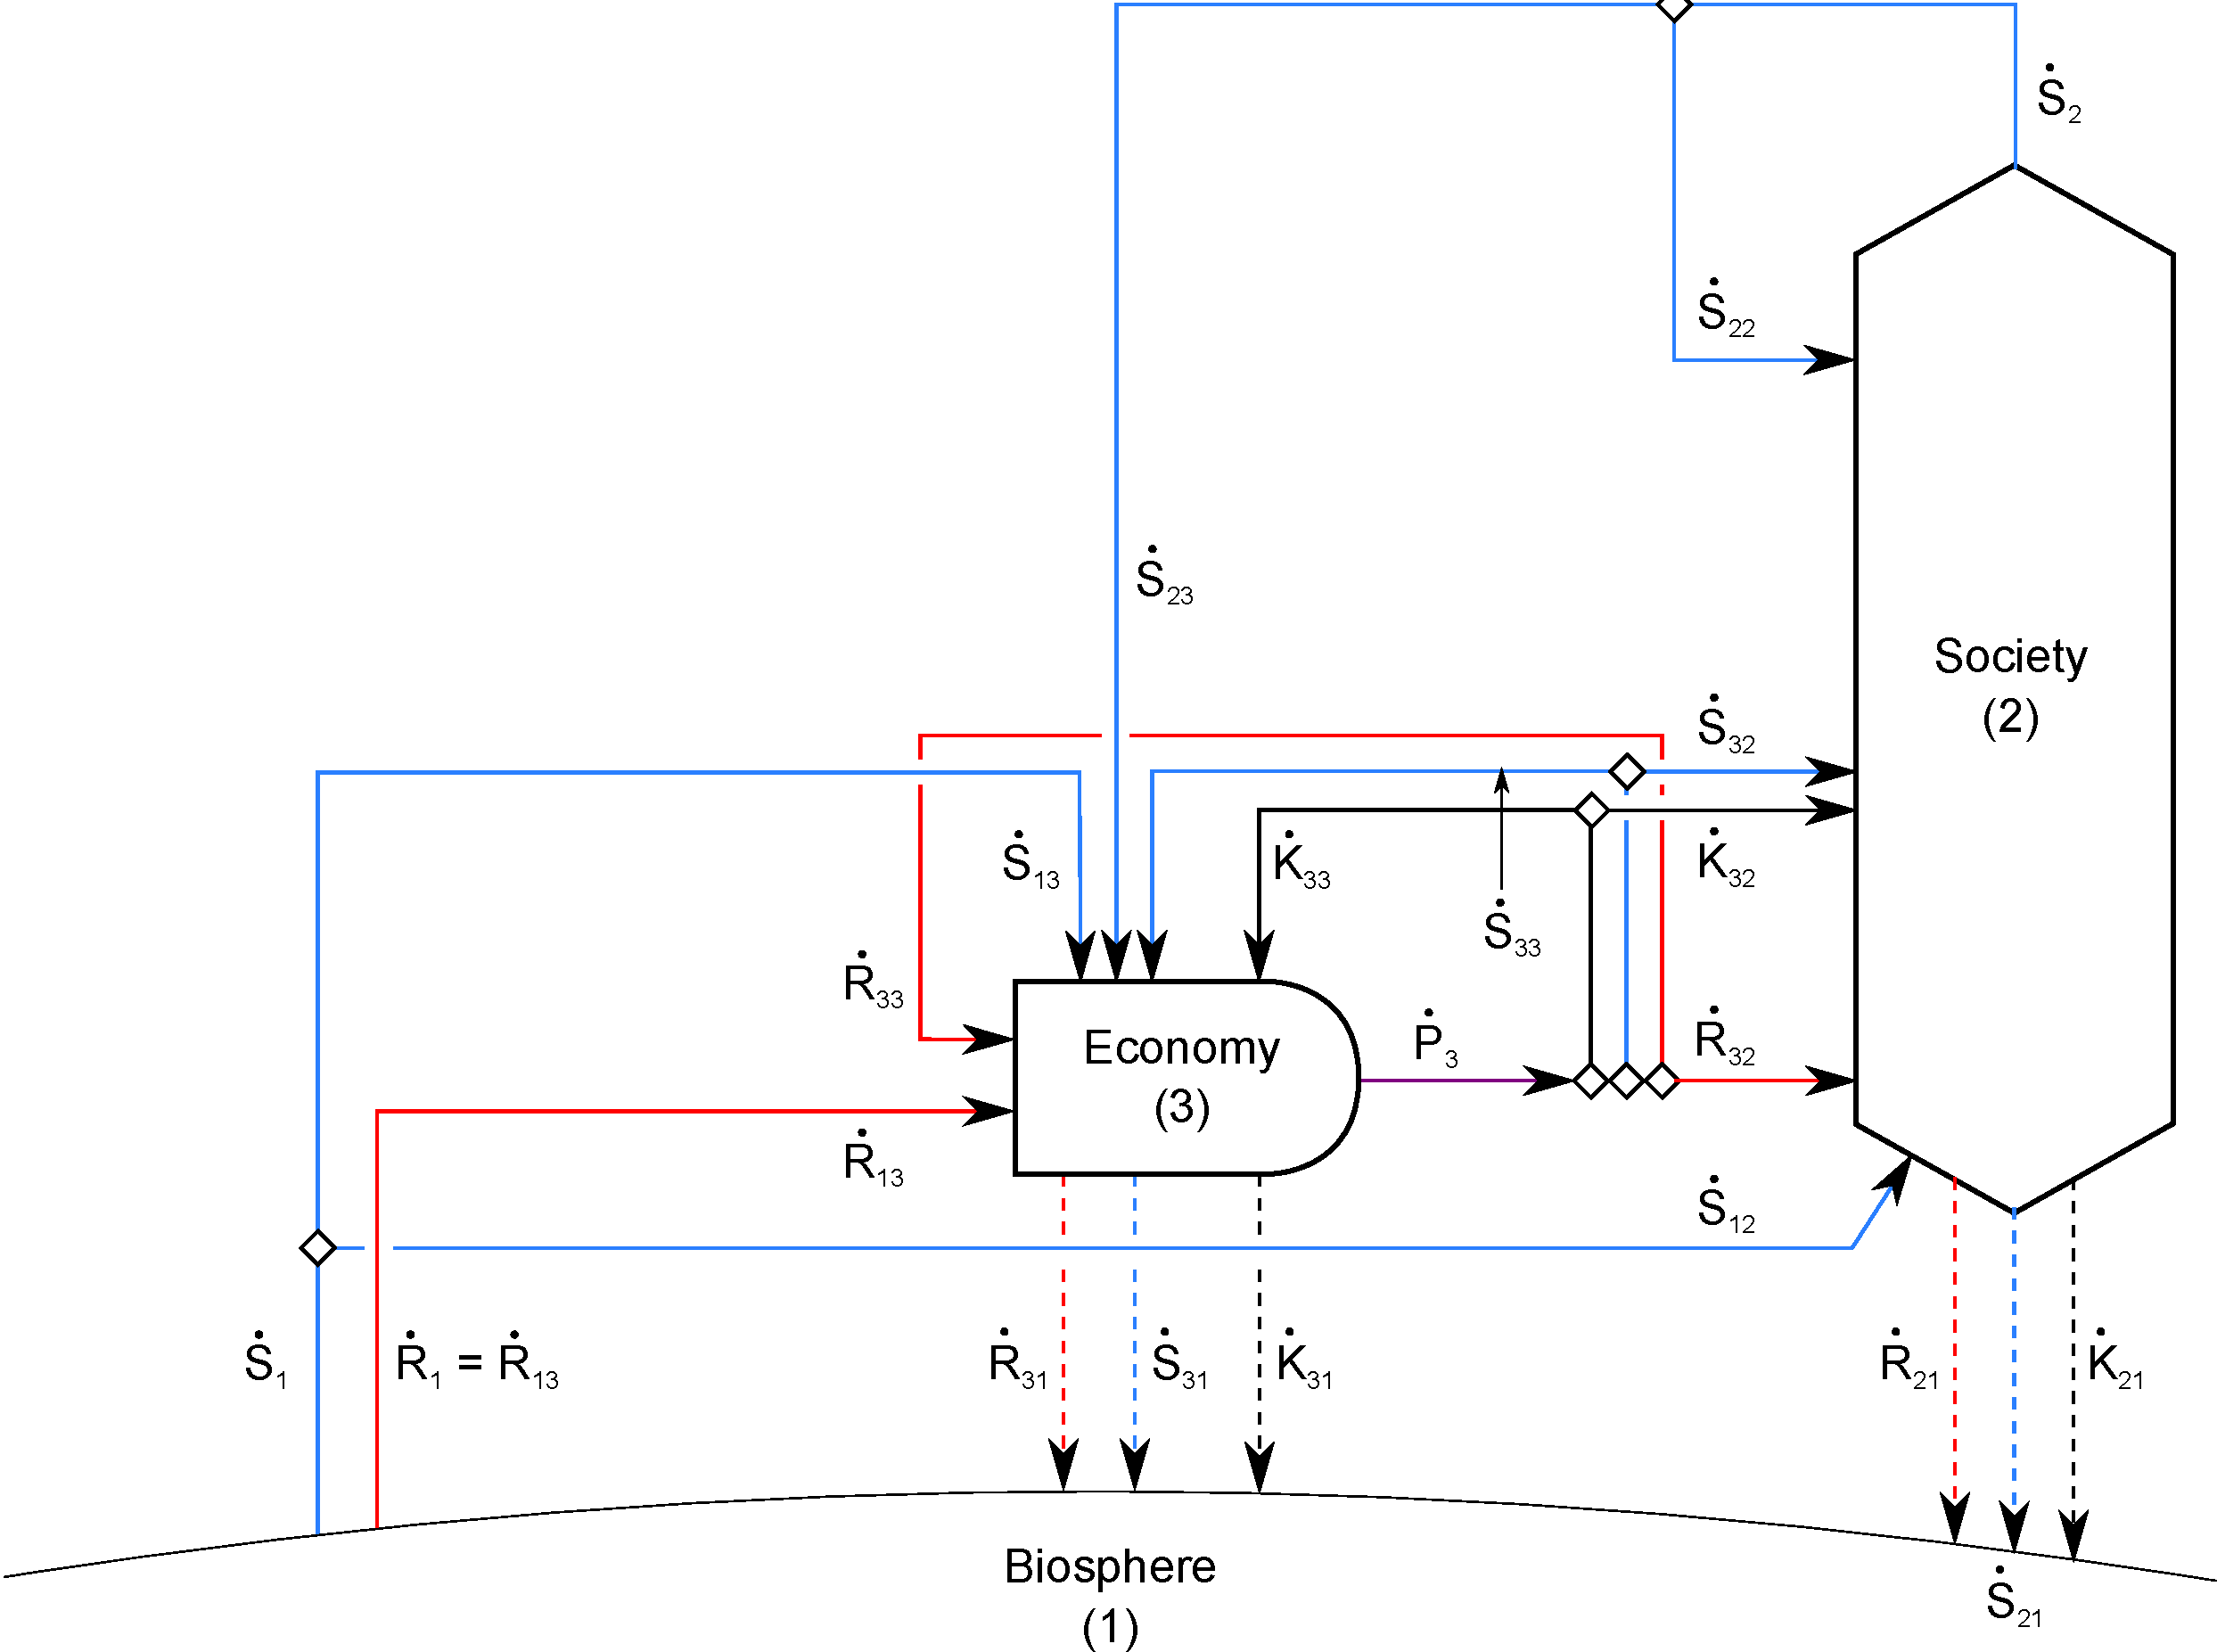
\includegraphics[width=0.8\linewidth]{Part_1/Chapter_Materials/images/2_sector_materials.pdf}
\caption[Flows of materials for a two-sector economy]{Flows of materials for a two-sector economy}
\label{fig:B_materials}
\end{figure}

As can be seen in Figure~\ref{fig:B_materials}, 
Sector~(2) resembles very closely the basic unit
outlined in Figure~\ref{fig:PERKS_materials}. 
Resource flows from the biosphere ($\dot{R}_{02}$)
and those produced by Sector~(2) itself ($\dot{R}_{22}$) 
are \emph{transformed} into product flow
($\dot{P}_{2}$). 
Flows of short-lived goods ($\dot{S}$) 
and capital ($\dot{K}$) are required to
support this transformative process. 
Much of the product flow from Sector~(2) 
enters final consumption (1) as resource ($\dot{R}_{21}$), 
short-lived good ($\dot{S}_{21}$) 
and capital good ($\dot{K}_{21}$)
flows.
% \footnote{This is a somewhat different conception of ``capital goods'' than is often used by
% economists, wherein capital goods are used only within production sectors of the economy. What we
% are here labelling as ``capital goods'' might be termed \emph{consumer durables} by economists. For
% our intention, consumer durables in society serve the same purpose as capital equipment in the
% economy---they are necessary to support the goal of the sector: production in one case
% and consumption in the other. [MAYBE REPHRASE AS ``production of goods in one case and production
% of labor in the other.'']}

There is also a product outflow 
from final consumption ($\dot{P}_{1}$), 
some of which is returned to final consumption
as resource ($\dot{R}_{11}$), 
short-lived good ($\dot{S}_{11}$) 
and capital good ($\dot{K}_{11}$) flows. 
A flow of short-lived goods ($\dot{S}_{12}$)
flows from final consumption (1) to production (2) 
associated with the flow of labor. 
There is no resource ($\dot{R}_{12}$) nor 
capital good ($\dot{K}_{12}$) flow from 
society (1) to production (2). 
This is because the `product' of final consumption
is the production of labor services 
and the ``consumption'' of final goods. 
No materials flow from final consumption to be 
\emph{transformed} into or \emph{embodied} 
in the production goods of Sector~(2), 
therefore $\dot{R}_{12} = 0$. 
Additionally, no capital \emph{goods} flow 
from final consumption to accumulate
within the production sector, 
therefore $\dot{K}_{12} = 0$.

% **** Rewrite this paragraph below ****


The short-lived goods flow ($\dot{S}_{12}$)
from final consumption to the production sector 
represents labor,
specifically  the material flow 
associated with labor's energy 
which is used within the production sector.
\footnote{We assume that this flow is the 
adenosine triphosphate (ATP), 
used as an energy
carrier within the cells of organisms.} 

As in Example~A, 
we set control volumes around the biosphere\index{biosphere} 
and our two economic sectors, 
such that the material accounting equations become:

\begin{align} 
\label{eq:B_CV_0}
	\frac{\mathrm{d}R_{0}}{\mathrm{d}t} 
	+ \frac{\mathrm{d}S_{0}}{\mathrm{d}t}	
	+ \frac{\mathrm{d}K_0}{\mathrm{d}t}		&
	=  \dot{R}_{10} + \dot{R}_{20} 
	+ \dot{S}_{10} + \dot{S}_{20} 
	+ \dot{K}_{10} + \dot{K}_{20} 
	- \dot{R}_{0} 
	- \dot{S}_{0} 							\\
\label{eq:B_CV_1}
	\frac{\mathrm{d}R_{1}}{\mathrm{d}t} 
	+ \frac{\mathrm{d}S_{1}}{\mathrm{d}t}	
	+ \frac{\mathrm{d}K_{1}}{\mathrm{d}t}	&
	=  \dot{R}_{11} 
	+ \dot{R}_{21}
	+ \dot{S}_{01} 
	+ \dot{S}_{11} 
	+ \dot{S}_{21}
	+ \dot{K}_{11}
	+ \dot{K}_{21}
	- \dot{P}_{1} 
	- \dot{R}_{10} 
	- \dot{S}_{10} 
	- \dot{K}_{10},							\\
\label{eq:B_CV_2}
	\frac{\mathrm{d}R_{2}}{\mathrm{d}t} 
	+ \frac{\mathrm{d}S_{2}}{\mathrm{d}t}
	+ \frac{\mathrm{d}K_{2}}{\mathrm{d}t}	&
	=  \dot{R}_{02} 
	+ \dot{R}_{22} 
	+ \dot{S}_{02} 
	+ \dot{S}_{12} 
	+ \dot{S}_{22} 
	+ \dot{K}_{22}
	- \dot{P}_{2}
	- \dot{R}_{20} 
	- \dot{S}_{20} 
	- \dot{K}_{20},
\end{align}

One point worth noting is that 
what we are here denoting as a flow of 
`capital goods'\index{capital goods}
into final consumption ($\dot{K}_{21}$) 
would more normally be referred to by economist as 
`consumer durables', 
though would also include other products, 
such as housing. 
The important concept being that some goods 
(fridges, televisions, apartment blocks) 
may accumulate within sector~(1)
and would be represented within flow 
$\dot{K}_{21}$, 
whereas other short-lived goods
(newspapers, plastic packaging, electricity) 
do not accumulate and are represented within flow 
$\dot{S}_{21}$.

Resource flow $\dot{R}_{21}$ 
into final consumption represents 
the material flow that will be embodied within the 
`product' of final consumption---human labor---
i.e.\ food produced by the agriculture industry
 %[WE NEED TO DISCUSS IF WE WANT TO ACCOUNT IT IN THIS WAY]
Since no resources flow directly to final consumption 
from the biosphere\footnote{A counter-example
to this assumption is the production of food
outside of the agricultural industry, 
i.e.\ by households. 
This may be large in agrarian economies.}
\index{biosphere}, we may say:

\begin{equation}\label{eq:B_R0}
	\dot{R}_{0} = \dot{R}_{02}.
\end{equation}

In contrast, 
short-lived materials may flow directly to final consumption 
from the biosphere\index{biosphere}, 
e.g.\ the flow of photons in sunlight or oxygen into car engines and lungs. 
We can redefine flows $\dot{S}_{0}$ and $\dot{S}_{1}$:

\begin{equation}\label{eq:B_S0}
	\dot{S}_{0} 
	= \dot{S}_{01} + \dot{S}_{02};
\end{equation}

As in Example A, we may easily define 
the balance of resources ($\dot{R}$),
short-lived materials ($\dot{S}$) and
capital ($\dot{K}$) within the biosphere:

\begin{align}\label{eq:B_dR0}
	\frac{\mathrm{d}R_{0}}{\mathrm{d}t}	&
	= \dot{R}_{10}
	+ \dot{R}_{20}
	- \dot{R}_{02},										\\
\label{eq:B_dS0}
	\frac{\mathrm{d}S_{0}}{\mathrm{d}t}	&
	= \dot{S}_{10}
	+ \dot{S}_{20}
	- \dot{S}_{01}
	- \dot{S}_{02},										\\	
\label{eq:B_dK0}
	\frac{\mathrm{d}K_{0}}{\mathrm{d}t}	&
	= \dot{K}_{10}
	+ \dot{K}_{20}.
\end{align}

Since we are assuming that only man-made capital
is accounted within the physical stock of final consumption\footnote{If
we were assuming that the human population
was accounted within $\dot{K}_{1}$,
then the `product' of final consumption would be human beings
(and the labor they provide),
resource flow $\dot{R}_{11}$ would be material resources
provided to human reproduction and
`capital goods' flow $\dot{K}_{11}$ would be material
added to the human population stock. Again, 
this issue is discussed in greater detail in 
Section~\ref{sec:people_as_stock}.}~($K_{1}$)
and that the `product' of final consumption is labor
(a short-lived material flow, $\dot{S}$),
then we may also state that:

\begin{equation}\label{eq:B_R11_K11}
	\dot{R}_{11} = \dot{K}_{11} = 0
\end{equation}

\noindent{}since all capital goods are produced within
the production sector (2).

% **** Are flows $\dot{R}_{11} = \dot{K}_{11} = 0$ *****
% **** Yes, they are, since we are assuming that
% $K_{1}$ includes only man-made capital, not humans
% and all capital manufacture occurs in 
% the production sector.

% [NOT SURE IF THIS IS TRUE IF WE THINK OF $\dot{R}_{12}$ AS FOOD AND $K_{1}$ 
% AS INCLUDING HUMANS\ldots 
% YES, I THINK $\dot{R}_{12}$ CAN BE TURNED INTO  $\dot{K}_{1}$ INTERNALLY, 
% AS THE ACCUMULATION OF (LITERAL) HUMAN CAPITAL, I.E. POPULATION]



From conservation of mass,
we can also define product flows
$\dot{P}_{1}$ and $\dot{P}_{2}$ as:

\begin{align}
\label{eq:B_P1_def}
	\dot{P}_{1}				&
	= \dot{S}_{11}
	+ \dot{S}_{12},			\\
\label{eq:B_P2_def}
	\dot{P}_{2}				&
	= \dot{R}_{21}
	+ \dot{R}_{22}
	+ \dot{S}_{21}
	+ \dot{S}_{22}
	+ \dot{K}_{21}	 
	+ \dot{K}_{22},
\end{align}


\noindent Again, remembering that resources and short-lived
goods do not accumulate within any sectors of the economy:

\begin{equation}\label{eq:dR_and_dS_zero}
	\frac{\mathrm{d}R_{1}}{\mathrm{d}t}
	= \frac{\mathrm{d}R_{2}}{\mathrm{d}t} 
	= \frac{\mathrm{d}S_{1}}{\mathrm{d}t} 
	= \frac{\mathrm{d}S_{2}}{\mathrm{d}t} 
	= 0,
\end{equation}

As in Example~A,
we may also define the resource-product
and short-lived goods flows balances separately
for each of the sectors of the economy:

\begin{align}
	\frac{\mathrm{d}R_{1}}{\mathrm{d}t} 	&
	= \dot{R}_{21}
	- \dot{P}_{1}
	- \dot{R}_{10}
	= 0,															\\
\label{eq:B_dS1}
	\frac{\mathrm{d}S_{1}}{\mathrm{d}t} 	&
	= \dot{S}_{01}
	+ \dot{S}_{11}
	+ \dot{S}_{21}
	- \dot{S}_{10}
	= 0,															\\
	\frac{\mathrm{d}R_{2}}{\mathrm{d}t} 	&
	= \dot{R}_{02}
	+ \dot{R}_{22}
	- \dot{P}_{2}
	- \dot{R}_{20}
	= 0,															\\
\label{eq:B_dS2}
	\frac{\mathrm{d}S_{2}}{\mathrm{d}t} 	&
	= \dot{S}_{02}
	+ \dot{S}_{12}
	+ \dot{S}_{22}
	- \dot{S}_{20}
	= 0,
\end{align}

We may rearrange these equations in terms of
the important variable.

\begin{align}
\label{eq:B_P1a}
	\dot{P}_{1}												&
	= \dot{R}_{21}
	- \dot{R}_{10}											\\
\label{eq:B_S11}
	\dot{S}_{11}											&
	= \dot{S}_{10}
	- \dot{S}_{21},										\\
\label{eq:B_P2a}
	\dot{P}_{2}												&
	= \dot{R}_{02}
	+ \dot{R}_{22}
	- \dot{R}_{20},										\\
\label{eq:B_S22}
	\dot{S}_{22}											&
	= \dot{S}_{20}
	- \dot{S}_{02} 
	- \dot{S}_{12}.	
\end{align}


Substituting
Equations~\ref{eq:B_R0}-\ref{eq:B_dK0}
into Equation~\ref{eq:B_CV_0}, 
we obtain:

\begin{align} \label{eq:B_CV_0a}
	\frac{\mathrm{d}R_{0}}{\mathrm{d}t} 
	+ \frac{\mathrm{d}S_{0}}{\mathrm{d}t}		& 
	= \dot{R}_{10} + \dot{R}_{20} 
	+ \dot{S}_{10} + \dot{S}_{20} 
	- \dot{R}_{02} 
	- \dot{S}_{01}
	- \dot{S}_{02}.
\end{align}

Substituting Equations~\ref{eq:dR_and_dS_zero},~\ref{eq:B_dS1}~and~\ref{eq:B_dS2}
into Equations~\ref{eq:B_CV_1}~and~\ref{eq:B_CV_2},
respectively,
we obtain:

\begin{align} 
\label{eq:B_CV_1a}
	 \frac{\mathrm{d}K_{1}}{\mathrm{d}t}	&
	=  \dot{R}_{21}
	+ \dot{K}_{21}
	- \dot{P}_{1} 
	- \dot{R}_{10} 
	- \dot{K}_{10},							\\
\label{eq:B_CV_2a}
	\frac{\mathrm{d}K_{2}}{\mathrm{d}t}	&
	=  \dot{R}_{02} 
	+ \dot{R}_{22} 
	+ \dot{K}_{22}
	- \dot{P}_{2}
	- \dot{R}_{20} 
	- \dot{K}_{20},
\end{align}


As in Example~A,
we again have two definitions for $\dot{P}_{1}$
(Equations~\ref{eq:B_P1_def}~and~\ref{eq:B_P1a})
and $\dot{P}_{2}$ 
(Equations~\ref{eq:B_P2_def}~and~\ref{eq:B_P2a})
which may be substituted into
Equations~\ref{eq:B_CV_1a}~and~\ref{eq:B_CV_2a},
respectively. 
Let us start by substituting Equations~\ref{eq:B_P1a}~and~\ref{eq:B_P2a},
in which case we obtain:

\begin{align} 
\label{eq:B_CV_1b}
	 \frac{\mathrm{d}K_{1}}{\mathrm{d}t}	&
	= \dot{K}_{21}
	- \dot{K}_{10},							\\
\label{eq:B_CV_2b}
	\frac{\mathrm{d}K_{2}}{\mathrm{d}t}	&
	=  \dot{K}_{22}
	- \dot{K}_{20},
\end{align}

\noindent{}which tells us that accumulation 
of man-made capital ($K$) is dependent
only on inflows of capital goods into the 
sector~($\dot{K}_{2j}$) and depreciation
of capital to the biosphere ($\dot{K}_{j0}$).

Now, substituting
Equations~\ref{eq:B_P1_def}~and~\ref{eq:B_P2_def},
we obtain:

\begin{align} 
\label{eq:B_CV_1c}
	 \frac{\mathrm{d}K_{1}}{\mathrm{d}t}	&
	=  \dot{R}_{21}
	+ \dot{K}_{21}
	- \dot{S}_{11}
	- \dot{S}_{12} 
	- \dot{R}_{10} 
	- \dot{K}_{10},							\\
\label{eq:B_CV_2c}
	\frac{\mathrm{d}K_{2}}{\mathrm{d}t}	&
	=  \dot{R}_{02} 
	- \dot{R}_{21}
	- \dot{S}_{21}
	- \dot{S}_{22}
	- \dot{K}_{21}	 
	- \dot{R}_{20} 
	- \dot{K}_{20},
\end{align}

\noindent{}to which we may make the 
substitution of the depreciation term (as before)
and rearrange to obtain:

\begin{align} 
\label{eq:B_CV_1d}
	- \dot{R}_{10} 	 										&
	 = \frac{\mathrm{d}K_{1}}{\mathrm{d}t}
	-  \dot{R}_{21}
	- \dot{K}_{21}
	+ \dot{S}_{11}
	+ \dot{S}_{12} 
	+ \gamma_{K_{1}}K_{1},											\\
\label{eq:B_CV_2d}
	\dot{R}_{02}
	- \dot{R}_{20} 											&
	= \frac{\mathrm{d}K_{2}}{\mathrm{d}t}	
	+ \left(\dot{R}_{21}
	+ \dot{S}_{21}
	+ \dot{K}_{21}\right)	 
	+ \dot{S}_{22}
	+ \gamma_{K_{2}}K_{2}.
\end{align}

Equation~\ref{eq:B_CV_2d} tells us that the resources
extracted and used by 
the production sector~($\dot{R}_{02} - \dot{R}_{20}$)
are for the purpose of:

\begin{itemize}
	\item building up capital stock
	in the production sector
	$\left(\frac{\mathrm{d}K_{2}}{\mathrm{d}t}\right)$
	\item manufactured goods 
	for final consumption
	$\left(\dot{R}_{21}
	+ \dot{S}_{21}
	+ \dot{K}_{21}\right)	$,
	\item providing short-lived goods
	to support the 
	production sector ($\dot{S}_{22}$), and
	\item overcoming depreciation of production 
	capital stock ($\gamma_{K_{2}}K_{2}$).
\end{itemize}

Adding these two equations together,
we obtain:

\begin{align} 
	- \frac{\mathrm{d}R_{0}}{\mathrm{d}t}			&
	= \dot{R}_{02}
	- \dot{R}_{10}
	- \dot{R}_{20}									\nonumber	\\
\label{eq:B_CV_1and2}											&
	= \frac{\mathrm{d}K_{1}}{\mathrm{d}t}
	+ \frac{\mathrm{d}K_{2}}{\mathrm{d}t}
	+ \dot{S}_{11}
	+ \dot{S}_{12} 
	+ \dot{S}_{21}
	+ \dot{S}_{22}
	+ \gamma_{K_{1}}K_{1}
	+ \gamma_{K_{2}}K_{2}.
\end{align}

\noindent{}which tells us that
the depletion of natural capital
$\left(\frac{\mathrm{d}R_{0}}{\mathrm{d}t}\right)$
is used within the economy in order to:

\begin{itemize}
	\item build up capital stock
	$\left(\frac{\mathrm{d}K_{1}}{\mathrm{d}t}
	+ \frac{\mathrm{d}K_{2}}{\mathrm{d}t}\right)$,
	\item produce short-lived goods
	($\dot{S}_{11}
	+ \dot{S}_{12} 
	+ \dot{S}_{21}
	+ \dot{S}_{22}$), and
	\item overcome depreciation
	$\left(\gamma_{K_{1}}K_{1}
	+ \gamma_{K_{2}}K_{2}\right)$.
\end{itemize}


%As in Equation~\ref{eq:A_dK_1/dt_b},
%we may define the disposal of man-made capital
%to the biosphere using a depreciation rate,
%such that:
%
%\begin{equation}\label{eq:B_CV_all_a}
%	\frac{\mathrm{d}K_{1}}{\mathrm{d}t}
%	+ \frac{\mathrm{d}K_{2}}{\mathrm{d}t}
%	= - \left(
%	\frac{\mathrm{d}R_{0}}{\mathrm{d}t} 
%	+ \frac{\mathrm{d}S_{0}}{\mathrm{d}t}	
%	\right)
%	- \gamma_{K_{1}}K_{1}
%	- \gamma_{K_{2}}K_{2}.
%\end{equation}
%
%Equation~\ref{eq:B_CV_all_a} states that 
%the accumulation of man-made capital
%within the production and final consumption sectors
%is equal to the depletion of natural resources
%less the depreciation of man-made capital to the biosphere.

%%%%%%%%%% Materials: Example C %%%%%%%%%%
\section{Example C: three-sector economy} % chktex 13
\label{sec:C_materials}
%%%%%%%%%%

In example C, we differentiate between two production sectors, sector (2) produces energy
products and sector (3) produces other goods and services, as depicted in Figure
\ref{fig:C_materials}.

\begin{figure}[!ht]
\centering
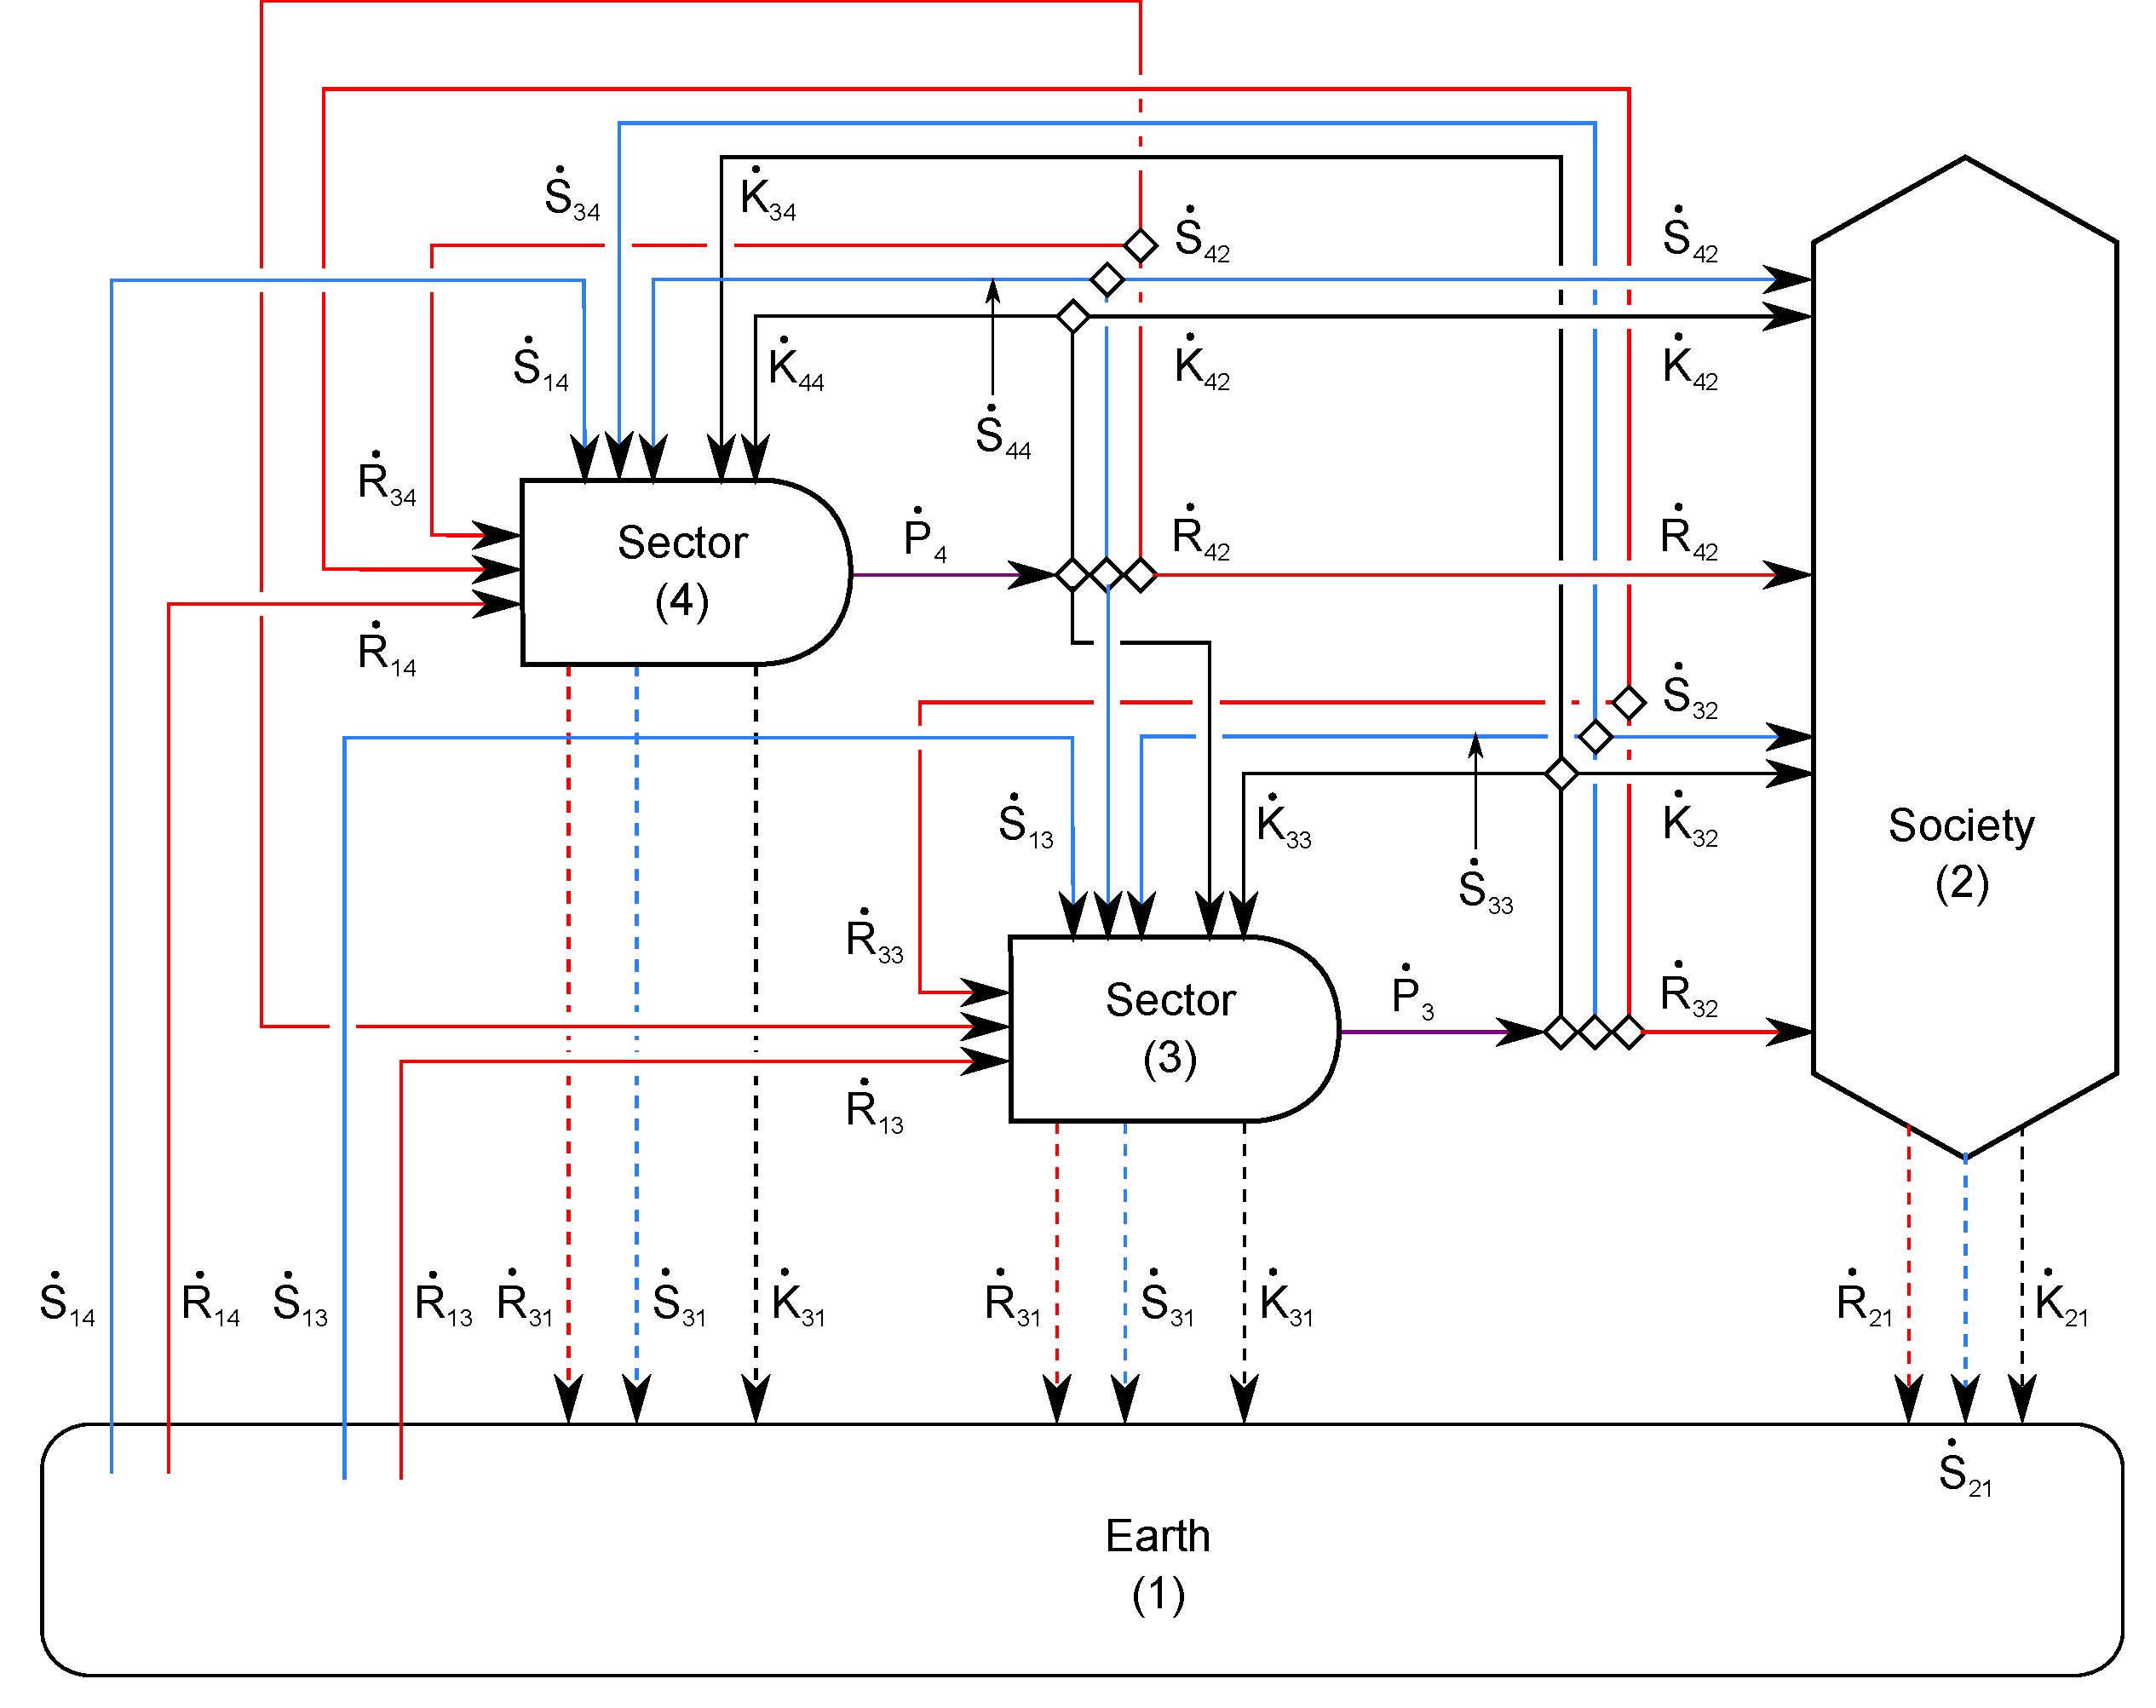
\includegraphics[width=0.8\linewidth]{Part_1/Chapter_Materials/images/3_sector_materials.pdf}
\caption[Flows of materials for a three-sector economy]{Flows of materials for a three-sector economy}
\label{fig:C_materials}
\end{figure}

In this example, we will take a slightly different approach
than in the previous two examples. 
Instead of discerning whether or not certain flows exist---asking for instance,
is there a flow of resources ($\dot{R}_{21}$) from
the energy sector (2) to final consumption (1)?----we
shall account for all flows,
\emph{even if} those flows are zero.
In this way,
we may build up a completely general
framework for material accounting within an economy
of any size.

Accounting for the material flows 
into and out of the biosphere\index{biosphere} 
(0) gives the following equation:

\begin{align} \label{eq:C_CV_0}
	\frac{\mathrm{d}R_{0}}{\mathrm{d}t} 
	+ \frac{\mathrm{d}S_{0}}{\mathrm{d}t}	
	+ \frac{\mathrm{d}K_0}{\mathrm{d}t}		
	& =  \dot{R}_{10} + \dot{R}_{20} + \dot{R}_{30}
	+ \dot{S}_{10} + \dot{S}_{20} + \dot{S}_{30}
	+ \dot{K}_{10} + \dot{K}_{20} + \dot{K}_{30}
	- \dot{R}_{0} 
	- \dot{S}_{0},
\end{align}

\noindent which may be rewritten as:

\begin{align} \label{eq:C_CV_0_b}
	\frac{\mathrm{d}R_{0}}{\mathrm{d}t} 
	+ \frac{\mathrm{d}S_{0}}{\mathrm{d}t}	
	+ \frac{\mathrm{d}K_0}{\mathrm{d}t}		
	& =  \sum_{i = 1}^{3}\dot{R}_{i0}
	+ \sum_{i = 1}^{3}\dot{S}_{i0}
	+ \sum_{i = 1}^{3}\dot{K}_{i0}
	- \dot{R}_{0} 
	- \dot{S}_{0},
\end{align}

Similarly, flows for the other sectors may be written:

\begin{align} \label{eq:C_CV_1}
	\frac{\mathrm{d}R_{1}}{\mathrm{d}t} 
	+ \frac{\mathrm{d}S_{1}}{\mathrm{d}t}	
	+ \frac{\mathrm{d}K_{1}}{\mathrm{d}t}		
	& =  \dot{R}_{01} 
	+ \dot{S}_{01}
	+ \sum_{i = 1}^{3}\dot{R}_{i1}
	+ \sum_{i = 1}^{3}\dot{S}_{i1}
	+ \sum_{i = 1}^{3}\dot{K}_{i1}
	- \dot{P}_{1}
	- \dot{R}_{10} 
	- \dot{S}_{10}
	- \dot{K}_{10},										\\
	\label{eq:C_CV_2}
	\frac{\mathrm{d}R_{2}}{\mathrm{d}t} 
	+ \frac{\mathrm{d}S_{2}}{\mathrm{d}t}	
	+ \frac{\mathrm{d}K_{2}}{\mathrm{d}t}		
	& =  \dot{R}_{02} 
	+ \dot{S}_{02}
	+ \sum_{i = 1}^{3}\dot{R}_{i2}
	+ \sum_{i = 1}^{3}\dot{S}_{i2}
	+ \sum_{i = 1}^{3}\dot{K}_{i2}
	- \dot{P}_{2}
	- \dot{R}_{20} 
	- \dot{S}_{20}
	- \dot{K}_{20},										\\	
	\label{eq:C_CV_3}
	\frac{\mathrm{d}R_{3}}{\mathrm{d}t} 
	+ \frac{\mathrm{d}S_{3}}{\mathrm{d}t}	
	+ \frac{\mathrm{d}K_{3}}{\mathrm{d}t}		
	& =  \dot{R}_{03} 
	+ \dot{S}_{03}
	+ \sum_{i = 1}^{3}\dot{R}_{i3}
	+ \sum_{i = 1}^{3}\dot{S}_{i3}
	+ \sum_{i = 1}^{3}\dot{K}_{i3}
	- \dot{P}_{3}
	- \dot{R}_{30} 
	- \dot{S}_{30}
	- \dot{K}_{30}.										
\end{align}

%Equations~\ref{eq:C_CV_1}~through~\ref{eq:C_CV_3} may be summarized
%in one single equation as:
%
%\begin{align} \label{eq:C_CV_1_to_3_b}
%	\frac{\mathrm{d}K_{j}}{\mathrm{d}t}		
%	& =  \dot{R}_{0j} 
%	+ \dot{S}_{0j}
%	+ \sum_{i = 1}^{3}\dot{R}_{ij}
%	+ \sum_{i = 1}^{3}\dot{S}_{ij}
%	+ \sum_{i = 1}^{3}\dot{K}_{ij}
%	- \dot{P}_{j}
%	- \dot{R}_{j0} 
%	- \dot{S}_{j0}
%	- \dot{K}_{j0};
%	& j \in \left[1,3\right].
%\end{align}

As in previous examples,
we may define the balance of 
resources~($\dot{R}$),
short-lived materials~($\dot{S}$) and
capital~($\dot{K}$) within the biosphere:

\begin{align}\label{eq:C_dR0}
	\frac{\mathrm{d}R_{0}}{\mathrm{d}t}	&
	= \dot{R}_{10}
	+ \dot{R}_{20}
	+ \dot{R}_{30}
	- \dot{R}_{01}
	- \dot{R}_{02}
	- \dot{R}_{03},										\\
\label{eq:C_dS0}
	\frac{\mathrm{d}S_{0}}{\mathrm{d}t}	&
	= \dot{S}_{10}
	+ \dot{S}_{20}
	+ \dot{S}_{30}	
	- \dot{S}_{01}
	- \dot{S}_{02}
	- \dot{S}_{03},										\\	
\label{eq:C_dK0}
	\frac{\mathrm{d}K_{0}}{\mathrm{d}t}	&
	= \dot{K}_{10}
	+ \dot{K}_{20}
	+ \dot{K}_{30}.
\end{align}

\noindent{}which may be rewritten:

\begin{align}
\label{eq:C_dR0a}
	\frac{\mathrm{d}R_{0}}{\mathrm{d}t}	&
	= \sum_{i = 1}^{3}\dot{R}_{i0}
	- \sum_{j = 1}^{3}\dot{R}_{0j},				\\
\label{eq:C_dS0a}
	\frac{\mathrm{d}S_{0}}{\mathrm{d}t}	&
	= \sum_{i = 1}^{3}\dot{S}_{i0}
	- \sum_{j = 1}^{3}\dot{S}_{0j},				\\
\label{eq:C_dK0a}
	\frac{\mathrm{d}K_{0}}{\mathrm{d}t}	&
	= \sum_{i = 1}^{3}\dot{K}_{i0}.
\end{align}

Applying conservation of mass
allows us to define the
product flows~($\dot{P}$) as:

\begin{align}
\label{eq:C_P1_def}
	\dot{P}_{1}										&
	= \sum_{j = 1}^{3}\dot{R}_{1j}
	+ \sum_{j = 1}^{3}\dot{S}_{1j}
	+ \sum_{j = 1}^{3}\dot{K}_{1j},	\\
\label{eq:C_P2_def}
	\dot{P}_{2}										&
	= \sum_{j = 1}^{3}\dot{R}_{2j}
	+ \sum_{j = 1}^{3}\dot{S}_{2j}
	+ \sum_{j = 1}^{3}\dot{K}_{2j},	\\
\label{eq:C_P3_def}							
	\dot{P}_{3}										&
	= \sum_{j = 1}^{3}\dot{R}_{3j}
	+ \sum_{j = 1}^{3}\dot{S}_{3j}
	+ \sum_{j = 1}^{3}\dot{K}_{3j}
\end{align}

As in Example~B, final consumption (1) provides 
only labor (represented by $\dot{S}$ flows)
to the other sectors of the economy.
The energy sector (2) provides 
energy products~($\dot{S}_{2j}$) to the other
sectors of the economy. 
It may also provide resources to itself ($\dot{R}_{22}$)
and to the goods and services sector (3), 
as in the case of metallurgical coke or 
natural gas for fertilizer.
The energy sector does not produce capital goods,
hence,
for $j \in [1,3]: \dot{K}_{2j} = 0$.
The goods and services (3) sector does not provide
resources for the energy sector (2)\footnote{There
may be some exceptions to this, as in the case of
energy from industrial waste streams.},
hence $\dot{R}_{32} = 0$.

Since we do not allow accumulation of either
resources~(R) or short-lived capital goods~(S) in
economic sectors,
then we may say:

\begin{equation}\label{eq:C_dR_and_dS_zero}
	\frac{\mathrm{d}R_{1}}{\mathrm{d}t}
	= \frac{\mathrm{d}R_{2}}{\mathrm{d}t} 
	= \frac{\mathrm{d}R_{3}}{\mathrm{d}t} 
	= \frac{\mathrm{d}S_{1}}{\mathrm{d}t} 
	= \frac{\mathrm{d}S_{2}}{\mathrm{d}t} 
	= \frac{\mathrm{d}S_{3}}{\mathrm{d}t} 
	= 0,
\end{equation}

As before,
we may also define the resource-product
and short-lived goods flows balances separately
for each of the sectors of the economy\footnote{It
is worth remembering here that 
$\dot{R}_{01} = \dot{R}_{21} = 0$,
since final consumption only takes resources
(in the form of food) from the goods and services
sector~(3) and that $R_{32} = 0$ since
the goods and services sector does not provide
resources to the energy sector~(2).}:

\begin{align}
	\frac{\mathrm{d}R_{1}}{\mathrm{d}t} 	&
	= \dot{R}_{01}
	+ \dot{R}_{11}
	+ \dot{R}_{21}
	+ \dot{R}_{31}
	- \dot{P}_{1}
	- \dot{R}_{10}
	= 0,															\\
\label{eq:C_dS1}
	\frac{\mathrm{d}S_{1}}{\mathrm{d}t} 	&
	= \dot{S}_{01}
	+ \dot{S}_{11}
	+ \dot{S}_{21}
	+ \dot{S}_{31}
	- \dot{S}_{10}
	= 0,															\\
	\frac{\mathrm{d}R_{2}}{\mathrm{d}t} 	&
	= \dot{R}_{02}
	+ \dot{R}_{12}
	+ \dot{R}_{22}
	+ \dot{R}_{32}
	- \dot{P}_{2}
	- \dot{R}_{20}
	= 0,															\\
\label{eq:C_dS2}
	\frac{\mathrm{d}S_{2}}{\mathrm{d}t} 	&
	= \dot{S}_{02}
	+ \dot{S}_{12}
	+ \dot{S}_{22}
	+ \dot{S}_{32}
	- \dot{S}_{20}
	= 0,															\\
	\frac{\mathrm{d}R_{3}}{\mathrm{d}t} 	&
	= \dot{R}_{03}
	+ \dot{R}_{13}
	+ \dot{R}_{23}
	+ \dot{R}_{33}
	- \dot{P}_{3}
	- \dot{R}_{30}
	= 0,															\\
\label{eq:C_dS3}
	\frac{\mathrm{d}S_{3}}{\mathrm{d}t} 	&
	= \dot{S}_{03}
	+ \dot{S}_{13}
	+ \dot{S}_{23}
	+ \dot{S}_{33}
	- \dot{S}_{30}
	= 0,
\end{align}

We may rearrange these equations
in terms of the important variable:

\begin{align}
\label{eq:C_P1a}
	\dot{P}_{1}												&
	= \dot{R}_{01}
	+ \dot{R}_{11}
	+ \dot{R}_{21}
	+ \dot{R}_{31}
	- \dot{R}_{10}											\\
\label{eq:C_S11}
	\dot{S}_{11}											&
	= \dot{S}_{10}
	- \dot{S}_{01}
	- \dot{S}_{21}
	- \dot{S}_{31},										\\
\label{eq:C_P2a}
	\dot{P}_{2}												&
	= \dot{R}_{02}
	+ \dot{R}_{12}
	+ \dot{R}_{22}
	+ \dot{R}_{32}
	- \dot{R}_{20},										\\
\label{eq:C_S22}
	\dot{S}_{22}											&
	= \dot{S}_{20}
	- \dot{S}_{02} 
	- \dot{S}_{12}
	- \dot{S}_{32},										\\
\label{eq:C_P3a}
	\dot{P}_{3}												&
	= \dot{R}_{03}
	+ \dot{R}_{13}
	+ \dot{R}_{23}
	+ \dot{R}_{33}
	- \dot{R}_{30},										\\
\label{eq:C_S33}
	\dot{S}_{33}											&
	= \dot{S}_{20}
	- \dot{S}_{03}
	- \dot{S}_{13}
	- \dot{S}_{23}.	
\end{align}

%We may rewrite Equation~\ref{eq:C_CV_0_b}
%by substituting 
%Equations~\ref{eq:C_dR0}~-~\ref{eq:C_dK0a}
%to obtain:
%
%\begin{align} \label{eq:C_CV_0_c}
%	\frac{\mathrm{d}R_{0}}{\mathrm{d}t} 
%	+ \frac{\mathrm{d}S_{0}}{\mathrm{d}t}	
%	& =  \sum_{i = 1}^{3}\dot{R}_{i0}
%	+ \sum_{i = 1}^{3}\dot{S}_{i0}
%	- \sum_{j = 2}^{3}\dot{R}_{0j}
%	- \sum_{j = 1}^{3}\dot{S}_{0j},
%\end{align}

We now make use of 
Equations~\ref{eq:C_dR_and_dS_zero},~\ref{eq:C_dS1},~\ref{eq:C_dS2}~and~\ref{eq:C_dS3},
in simplifying Equations~\ref{eq:C_CV_1}~-~\ref{eq:C_CV_3},
to obtain:

\begin{align} \label{eq:C_CV_1a}
	\frac{\mathrm{d}K_{1}}{\mathrm{d}t}		
	& =  \dot{R}_{01} 
	+ \sum_{i = 1}^{3}\dot{R}_{i1}
	+ \sum_{i = 1}^{3}\dot{K}_{i1}
	- \dot{P}_{1}
	- \dot{R}_{10} 
	- \dot{K}_{10},										\\
	\label{eq:C_CV_2a}
	\frac{\mathrm{d}K_{2}}{\mathrm{d}t}		
	& =  \dot{R}_{02} 
	+ \sum_{i = 1}^{3}\dot{R}_{i2}
	+ \sum_{i = 1}^{3}\dot{K}_{i2}
	- \dot{P}_{2}
	- \dot{R}_{20} 
	- \dot{K}_{20},										\\	
	\label{eq:C_CV_3a}
	\frac{\mathrm{d}K_{3}}{\mathrm{d}t}		
	& =  \dot{R}_{03} 
	+ \sum_{i = 1}^{3}\dot{R}_{i3}
	+ \sum_{i = 1}^{3}\dot{K}_{i3}
	- \dot{P}_{3}
	- \dot{R}_{30} 
	- \dot{K}_{30}.										
\end{align}

As in previous examples,
we have two different formulations for
the $\dot{P}$ terms.
Substituting, 
first, 
Equations~\ref{eq:C_P1a},~\ref{eq:C_P2a}~and~\ref{eq:C_P3a},
we obtain:

\begin{align} \label{eq:C_CV_1b}
	\frac{\mathrm{d}K_{1}}{\mathrm{d}t}		
	& = \sum_{i = 1}^{3}\dot{K}_{i1}
	- \dot{K}_{10},										\\
	\label{eq:C_CV_2b}
	\frac{\mathrm{d}K_{2}}{\mathrm{d}t}		
	& = \sum_{i = 1}^{3}\dot{K}_{i2}
	- \dot{K}_{20},										\\	
	\label{eq:C_CV_3b}
	\frac{\mathrm{d}K_{3}}{\mathrm{d}t}		
	& = \sum_{i = 1}^{3}\dot{K}_{i3}
	- \dot{K}_{30},										
\end{align}

\noindent{}which we may rewrite as the 
more general result:

\begin{align} \label{eq:C_CV_K_balance}
	\frac{\mathrm{d}K_{j}}{\mathrm{d}t}		
	& =  \sum_{i}\dot{K}_{ij}
	- \dot{K}_{j0}.
\end{align}

Equation~\ref{eq:C_CV_K_balance} states that
for any economic sector,
the accumulation of man-made capital stock
is dependent only on inflows of capital stock
from other economic sectors
($\dot{K}_{ij}$)
and depreciation of capital stock back to the
biosphere ($\dot{K}_{j0}$).

Instead,
substituting the alternative formulation for $\dot{P}$
from Equations~\ref{eq:C_P1_def}~-~\ref{eq:C_P3_def}
into Equations~\ref{eq:C_CV_1a}~-~\ref{eq:C_CV_3a},
respectively,
we obtain:

\begin{align} \label{eq:C_CV_1c}
	\frac{\mathrm{d}K_{1}}{\mathrm{d}t}	&
	= \dot{R}_{01}
	+ \sum_{i = 1}^{3}\dot{R}_{i1}
	+ \sum_{i = 1}^{3}\dot{K}_{i1}
	- \sum_{j = 1}^{3}\dot{R}_{1j}
	- \sum_{j = 1}^{3}\dot{S}_{1j}
	- \sum_{j = 1}^{3}\dot{K}_{1j}
	- \dot{R}_{10} 
	- \dot{K}_{10},										\\
	\label{eq:C_CV_2c}
	\frac{\mathrm{d}K_{2}}{\mathrm{d}t}	& 
	=  \dot{R}_{02} 
	+ \sum_{i = 1}^{3}\dot{R}_{i2}
	+ \sum_{i = 1}^{3}\dot{K}_{i2}
	- \sum_{j = 1}^{3}\dot{R}_{2j}
	- \sum_{j = 1}^{3}\dot{S}_{2j}
	- \sum_{j = 1}^{3}\dot{K}_{2j}
	- \dot{R}_{20} 
	- \dot{K}_{20},										\\	
	\label{eq:C_CV_3c}
	\frac{\mathrm{d}K_{3}}{\mathrm{d}t}	&
	=  \dot{R}_{03} 
	+ \sum_{i = 1}^{3}\dot{R}_{i3}
	+ \sum_{i = 1}^{3}\dot{K}_{i3}
	- \sum_{j = 1}^{3}\dot{R}_{3j}
	- \sum_{j = 1}^{3}\dot{S}_{3j}
	- \sum_{j = 1}^{3}\dot{K}_{3j}
	- \dot{R}_{30} 
	- \dot{K}_{30}.										
\end{align}

As before, we can rearrange these equations
to obtain:

\begin{align} \label{eq:C_CV_1d}
	\dot{R}_{01}
	- \dot{R}_{10} 											&
	=\frac{\mathrm{d}K_{1}}{\mathrm{d}t}
	- \sum_{i = 1}^{3}\dot{R}_{i1}
	- \sum_{i = 1}^{3}\dot{K}_{i1}
	+ \sum_{j = 1}^{3}\dot{R}_{1j}
	+ \sum_{j = 1}^{3}\dot{S}_{1j}
	+ \sum_{j = 1}^{3}\dot{K}_{1j}
	+ \dot{K}_{10},											\\
	\label{eq:C_CV_2d}
	\dot{R}_{02} 
	- \dot{R}_{20} 											&
	= \frac{\mathrm{d}K_{2}}{\mathrm{d}t}
	- \sum_{i = 1}^{3}\dot{R}_{i2}
	- \sum_{i = 1}^{3}\dot{K}_{i2}
	+ \sum_{j = 1}^{3}\dot{R}_{2j}
	+ \sum_{j = 1}^{3}\dot{S}_{2j}
	+ \sum_{j = 1}^{3}\dot{K}_{2j}
	+ \dot{K}_{20},											\\	
	\label{eq:C_CV_3d}
	\dot{R}_{03}
	- \dot{R}_{30} 											&
	= \frac{\mathrm{d}K_{3}}{\mathrm{d}t}
	- \sum_{i = 1}^{3}\dot{R}_{i3}
	- \sum_{i = 1}^{3}\dot{K}_{i3}
	+ \sum_{j = 1}^{3}\dot{R}_{3j}
	+ \sum_{j = 1}^{3}\dot{S}_{3j}
	+ \sum_{j = 1}^{3}\dot{K}_{3j}
	+ \dot{K}_{30}.										
\end{align}

Summing Equations~\ref{eq:C_CV_1d}~-~\ref{eq:C_CV_3d},
we obtain:

\begin{align}\label{eq:C_CV_all}
	- \frac{\mathrm{d}R_{0}}{\mathrm{d}t}										&
	= \sum_{j = 1}^{3}\dot{R}_{0j}
	- \sum_{i = 1}^{3}\dot{R}_{i0}									\nonumber	\\
	& =\frac{\mathrm{d}K_{1}}{\mathrm{d}t}
	+ \frac{\mathrm{d}K_{2}}{\mathrm{d}t}
	+ \frac{\mathrm{d}K_{3}}{\mathrm{d}t}
	- \sum_{j = 1}^{3}\sum_{i = 1}^{3}\dot{R}_{ij}
	- \sum_{j = 1}^{3}\sum_{i = 1}^{3}\dot{K}_{ij}
	+ \sum_{j = 1}^{3}\sum_{i = 1}^{3}\dot{R}_{ij}		\nonumber	\\
	& \qquad {} + \sum_{j = 1}^{3}\sum_{i = 1}^{3}\dot{S}_{ij}
	+ \sum_{j = 1}^{3}\sum_{i = 1}^{3}\dot{K}_{ij}
	+ \dot{K}_{10}
	+ \dot{K}_{20}
	+ \dot{K}_{30}.
\end{align}

\noindent{}which,
after substituting for 
the depreciation term ($\dot{K}_{i0}$),
simplifies to:

\begin{align}\label{eq:C_CV_all_a}
	- \frac{\mathrm{d}R_{0}}{\mathrm{d}t}										&
	=\sum_{j = 1}^{3}\frac{\mathrm{d}K_{j}}{\mathrm{d}t}
	+ \sum_{j = 1}^{3}\sum_{i = 1}^{3}\dot{S}_{ij}
	+ \sum_{j = 1}^{3}\gamma_{K_{j}}K_{j}
\end{align}

\noindent{}or,
more generally:

\begin{align}\label{eq:C_CV_all_b}
	- \frac{\mathrm{d}R_{0}}{\mathrm{d}t}										&
	=\sum_{j}\frac{\mathrm{d}K_{j}}{\mathrm{d}t}
	+ \sum_{i,j}\dot{S}_{ij}
	+ \sum_{j}\gamma_{K_{j}}K_{j}.
\end{align}

Similarly to what we saw in Examples~A~and~B,
Equation~\ref{eq:C_CV_all_b} tells us that,
depletion of natural resources in the 
biosphere~$\left(- \frac{\mathrm{d}R_{0}}{\mathrm{d}t}\right)$
by the economy
are used for the purposes of:

\begin{itemize}
	\item increasing man-made capital stocks
	within the economy~$\left(\frac{\mathrm{d}K_{j}}{\mathrm{d}t}\right)$
	\item providing short-lived goods exchanged within the
	economy~($\dot{S}_{ij}$), and
	\item overcoming depreciation of man-made
	capital stocks~($\sum_{j}\gamma_{K_{j}}K_{j}$).
\end{itemize}

\noindent{}This issue will be discussed in greater detail
in Section~\ref{sec:SSE} concerning 
sustainable scale of the economy and
the concept of a steady-state economy.

The exchange of resources ($\dot{R}$) and 
short-lived goods ($\dot{S}$) between 
each of the four `sectors' 
(the biosphere\index{biosphere} and 
the three economic sectors) 
may be thought of as four matrices 
(as depicted in Figure~\ref{fig:C_mat_matrix} 
for $\dot{S}$ flows): 
one $3\times3$ matrix of flows 
entirely within the economy, 
a $3\times1$ vector of flows from the 
biosphere\index{biosphere} into the economy (extraction), 
a $1\times3$ vector of flows from the economy 
into the biosphere\index{biosphere} (waste\index{waste}) 
and a $1\times1$ matrix of flows 
solely within the biosphere\index{biosphere} (environment), 
that do not enter the economy.

\begin{figure}[!ht]
\centering\
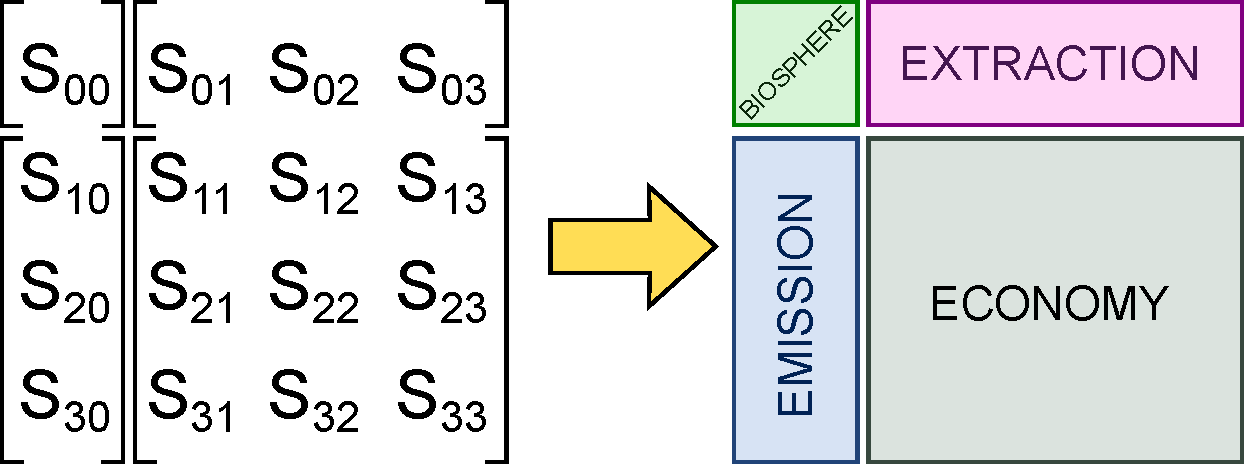
\includegraphics[width=0.8\linewidth]{Part_1/Chapter_Materials/images/Matrix.pdf}
\caption[The matrix of biosphere\index{biosphere}-economy flows.]{The matrix of biosphere-economy flows. 
}
\label{fig:C_mat_matrix}
\end{figure}

%%%%%%%%%% Materials: Auto industry example %%%%%%%%%%
\section{Materials in the auto industry}
\label{sec:materials_auto}
%%%%%%%%%%

Throughout the book, we shall be applying the methodology
that has been outlined through the examples to the
real-world case of the US auto industry.
In Figure~\ref{fig:PERKS_materials_auto}
we see the flows of resources,
short-lived and capital materials
into the auto industry.
Because the industry does not
extract resources directly from the biosphere,
the rate of flow of resources ($\dot{R}$) 
from the biosphere to the auto industry 
has a zero value.
Each of the other flows represented in the diagram is,
in actuality,
a vector of hundreds (or even thousands!)
of elemental material flows,
each of which must be accounted 
(and balanced) separately.

**** MCD---Talk about the different materials:
steel, glass, rubber, concrete, electricity, plastic
finished product is automobile. 
Emissions to air and water.
Talk to financial (value) flows in Section~\ref{sec:value_auto} 
as proxy for physical flows****

Data on the rest of the flows at the industry level
is very hard to obtain.
In Europe,
economy-wide material flow accounts (EW-MFA)
have been produced for each of the member 
states.\cite{EUROSTAT2011} 
Work is ongoing to characterize the inter-sectoral
flows of materials.\cite{ConAccount1998}

A number of studies have looked at 
the material and energy flows 
associated with vehicle manufacturing 
processes.\cite{MacLean1998,McCleese2002,MacLean2003}
The US automobile industry is composed
of many of these manufacturing processes.
In theory,
a representation of the industry-level flows
could be ``built up'' by assuming that the results from
these process-based models represent average
processes within the whole industry and 
scaling the material flows accordingly,
with appropriately wide uncertainty bounds.


**** MCD---I'm not sure what else I can write here.
% I could talk about process-based models? 
Talk about other industries
that may have better data.
Signpost the issue of lack of data in Section~\ref{sec:Data}
****

\begin{figure}[!ht]
\centering
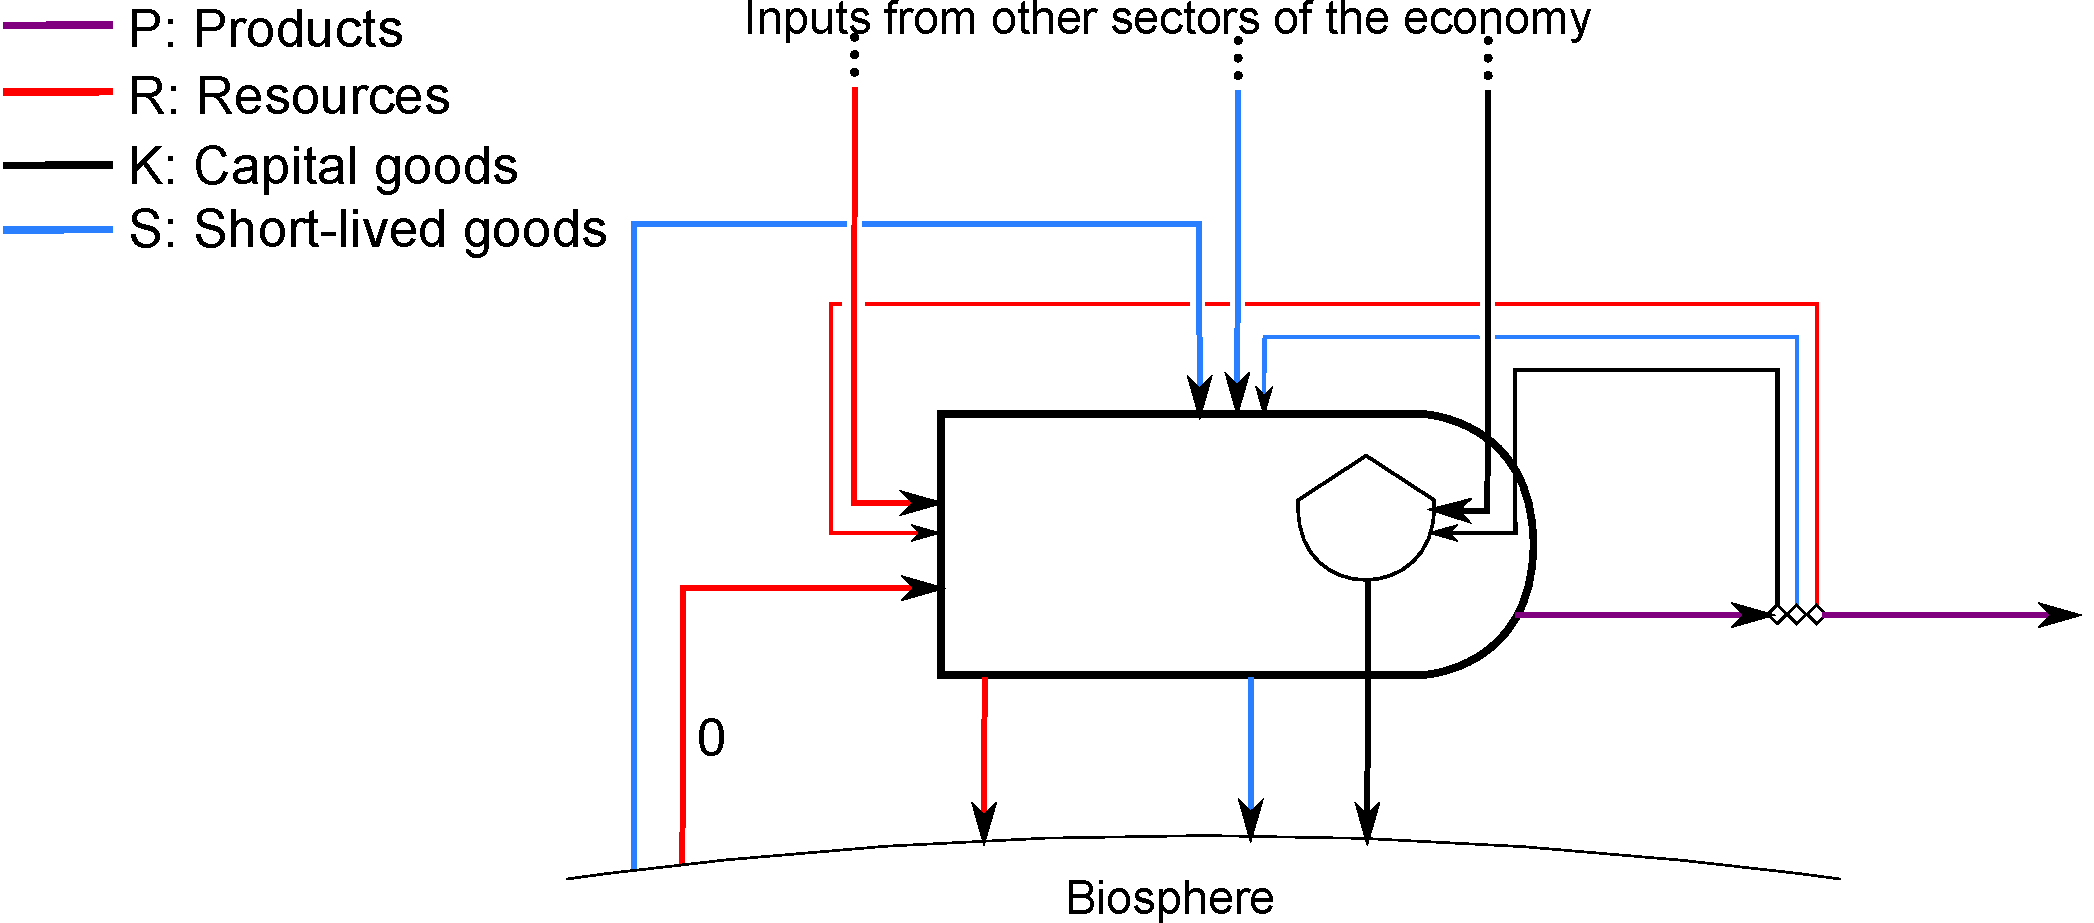
\includegraphics[width=0.8\linewidth]{Part_1/Chapter_Materials/images/PERKS_basic_unit_materials_auto_ind.pdf}
\caption[Material flows for the US Automobile Industry]{Material flows for the US Automobile Industry using data from XXXX}
\label{fig:PERKS_materials_auto}
\end{figure}

%%%%%%%%%% Materials: Summary %%%%%%%%%%
\section{Summary}
\label{sec:materials_summary}
%%%%%%%%%%

\bibliographystyle{unsrt}
\bibliography{../../EROI_review_v2}


% Always give a unique label
% and use \ref{<label>} for cross-references
% and \cite{<label>} for bibliographic references
% use \sectionmark{}
% to alter or adjust the section heading in the running head
%% Instead of simply listing headings of different levels we recommend to let every heading be followed by at least a short passage of text. Furtheron please use the \LaTeX\ automatism for all your cross-references and citations.

%% Please note that the first line of text that follows a heading is not indented, whereas the first lines of all sequent paragraphs are.

%% Use the standard \verb|equation| environment to typeset your equations, e.g.
%
%% \begin{equation}
%% a \times b = c\;,
%% \end{equation}
%
%% however, for multiline equations we recommend to use the \verb|eqnarray|
%% environment\footnote{In physics texts please activate the class option \texttt{vecphys} to depict your vectors in \textbf{\itshape boldface-italic} type - as is customary for a wide range of physical jects.}.
%%\begin{eqnarray}
%%a \times b = c \nonumber\\
%% \vec{a} \cdot \vec{b}=\vec{c}
%% \label{eq:01}
%%\end{eqnarray}

%% \section{section Heading}
%% \label{sec:2}
%% Instead of simply listing headings of different levels we recommend to let every heading be followed by at least a short passage of text. Furtheron please use the \LaTeX\ automatism for all your cross-references\index{cross-references} and citations\index{citations} as has already been described in Sect.~\ref{sec:2}.

%% \begin{quotation}
%% Please do not use quotation marks when quoting texts! Simply use the \verb|quotation| environment -- it will automatically render Springer's preferred layout.
%% \end{quotation}


%% \section{section Heading}
%% Instead of simply listing headings of different levels we recommend to let every heading be followed by at least a short passage of text. Furtheron please use the \LaTeX\ automatism for all your cross-references and citations as has already been described in Sect.~\ref{sec:2}, see also Fig.~\ref{fig:1}\footnote{If you copy text passages, figures, or tables from other works, you must obtain \textit{permission} from the copyright holder (usually the original publisher). Please enclose the signed permission with the manucript. The sources\index{permission to print} must be acknowledged either in the captions, as footnotes or in a separate section of the book.}

%% Please note that the first line of text that follows a heading is not indented, whereas the first lines of all sequent paragraphs are.

% For figures use
%
%% \begin{figure}[b]
%% \sidecaption
% Use the relevant command for your figure-insertion program
% to insert the figure file.
% For example, with the option graphics use
%% \includegraphics[scale=.65]{figure}
%
% If not, use
%\picplace{5cm}{2cm} % Give the correct figure height and width in cm
%
%% \caption{If the width of the figure is less than 7.8 cm use the \texttt{sidecapion} command to flush the caption on the left side of the page. If the figure is positioned at the top of the page, align the sidecaption with the top of the figure -- to achieve this you simply need to use the optional argument \texttt{[t]} with the \texttt{sidecaption} command}
%% \label{fig:1}       % Give a unique label
%% \end{figure}


%% \paragraph{Paragraph Heading} %
%% Instead of simply listing headings of different levels we recommend to let every heading be followed by at least a short passage of text. Furtheron please use the \LaTeX\ automatism for all your cross-references and citations as has already been described in Sect.~\ref{sec:2}.

%% Please note that the first line of text that follows a heading is not indented, whereas the first lines of all sequent paragraphs are.

%% For typesetting numbered lists we recommend to use the \verb|enumerate| environment -- it will automatically render Springer's preferred layout.

%% \begin{enumerate}
%% \item{Livelihood and survival mobility are oftentimes coutcomes of uneven socioeconomic development.}
%% \begin{enumerate}
%% \item{Livelihood and survival mobility are oftentimes coutcomes of uneven socioeconomic development.}
%% \item{Livelihood and survival mobility are oftentimes coutcomes of uneven socioeconomic development.}
%% \end{enumerate}
%% \item{Livelihood and survival mobility are oftentimes coutcomes of uneven socioeconomic development.}
%% \end{enumerate}


%% \paragraph{paragraph Heading} In order to avoid simply listing headings of different levels we recommend to let every heading be followed by at least a short passage of text. Use the \LaTeX\ automatism for all your cross-references and citations as has already been described in Sect.~\ref{sec:2}, see also Fig.~\ref{fig:2}.

%% Please note that the first line of text that follows a heading is not indented, whereas the first lines of all sequent paragraphs are.

%% For unnumbered list we recommend to use the \verb|itemize| environment -- it will automatically render Springer's preferred layout.

%% \begin{itemize}
%% \item{Livelihood and survival mobility are oftentimes coutcomes of uneven socioeconomic development, cf. Table~\ref{tab:1}.}
%% \begin{itemize}
%% \item{Livelihood and survival mobility are oftentimes coutcomes of uneven socioeconomic development.}
%% \item{Livelihood and survival mobility are oftentimes coutcomes of uneven socioeconomic development.}
%% \end{itemize}
%% \item{Livelihood and survival mobility are oftentimes coutcomes of uneven socioeconomic development.}
%% \end{itemize}

%% \begin{figure}[t]
%% \sidecaption[t]
% Use the relevant command for your figure-insertion program
% to insert the figure file.
% For example, with the option graphics use
%% \includegraphics[scale=.65]{figure}
%
% If not, use
%\picplace{5cm}{2cm} % Give the correct figure height and width in cm
%
%% \caption{Please write your figure caption here}
%% \label{fig:2}       % Give a unique label
%% \end{figure}

%% \runinhead{Run-in Heading Boldface Version} Use the \LaTeX\ automatism for all your cross-references and citations as has already been described in Sect.~\ref{sec:2}.

%% \runinhead{Run-in Heading Italic Version} Use the \LaTeX\ automatism for all your cross-refer\-ences and citations as has already been described in Sect.~\ref{sec:2}\index{paragraph}.
% Use the \index{} command to code your index words
%
% For tables use
%
%% \begin{table}
%% \caption{Please write your table caption here}
%% \label{tab:1}       % Give a unique label
%
% For LaTeX tables use
%
%% \begin{tabular}{p{2cm}p{2.4cm}p{2cm}p{4.9cm}}
%% \hline\noalign{\smallskip}
%% Classes & class & Length & Action Mechanism  \\
%% \noalign{\smallskip}\svhline\noalign{\smallskip}
%% Translation & mRNA$^a$  & 22 (19--25) & Translation repression, mRNA cleavage\\
%% Translation & mRNA cleavage & 21 & mRNA cleavage\\
%% Translation & mRNA  & 21--22 & mRNA cleavage\\
%%Translation & mRNA  & 24--26 & Histone and DNA Modification\\
%%\noalign{\smallskip}\hline\noalign{\smallskip}
%%\end{tabular}
%%$^a$ Table foot note (with superscript)
%%\end{table}
%
%% \section{Section Heading}
%%\label{sec:3}
% Always give a unique label
% and use \ref{<label>} for cross-references
% and \cite{<label>} for bibliographic references
% use \sectionmark{}
% to alter or adjust the section heading in the running head
%% Instead of simply listing headings of different levels we recommend to let every heading be followed by at least a short passage of text. Furtheron please use the \LaTeX\ automatism for all your cross-references and citations as has already been described in Sect.~\ref{sec:2}.

%% Please note that the first line of text that follows a heading is not indented, whereas the first lines of all sequent paragraphs are.

%%If you want to list definitions or the like we recommend to use the Springer-enhanced \verb|description| environment -- it will automatically render Springer's preferred layout.

%%\begin{description}[Type 1]
%%\item[Type 1]{That addresses central themes pertainng to migration, health, and disease. In Sect.~\ref{sec:1}, Wilson discusses the role of human migration in infectious disease distributions and patterns.}
%%\item[Type 2]{That addresses central themes pertainng to migration, health, and disease. In Sect.~\ref{sec:2}, Wilson discusses the role of human migration in infectious disease distributions and patterns.}
%%\end{description}

%%\section{section Heading} %
%% In order to avoid simply listing headings of different levels we recommend to let every heading be followed by at least a short passage of text. Use the \LaTeX\ automatism for all your cross-references and citations citations as has already been described in Sect.~\ref{sec:2}.

%% Please note that the first line of text that follows a heading is not indented, whereas the first lines of all sequent paragraphs are.

%% \begin{svgraybox}
%% If you want to emphasize complete paragraphs of texts we recommend to use the newly defined Springer class option \verb|graybox| and the newly defined environment \verb|svgraybox|. This will produce a 15 percent screened box 'behind' your text.

%% If you want to emphasize complete paragraphs of texts we recommend to use the newly defined Springer class option and environment \verb|svgraybox|. This will produce a 15 percent screened box 'behind' your text.
%% \end{svgraybox}


%% \section{section Heading}
%%Instead of simply listing headings of different levels we recommend to let every heading be followed by at least a short passage of text. Furtheron please use the \LaTeX\ automatism for all your cross-references and citations as has already been described in Sect.~\ref{sec:2}.

%% Please note that the first line of text that follows a heading is not indented, whereas the first lines of all sequent paragraphs are.

%% \begin{theorem}
%% Theorem text goes here.
%% \end{theorem}
%
% or
%
%% \begin{definition}
%% Definition text goes here.
%% \end{definition}

%% \begin{proof}
%\smartqed
%% Proof text goes here.
%% \qed
%% \end{proof}

%%\paragraph{Paragraph Heading} %
%% Instead of simply listing headings of different levels we recommend to let every heading be followed by at least a short passage of text. Furtheron please use the \LaTeX\ automatism for all your cross-references and citations as has already been described in Sect.~\ref{sec:2}.

%% Note that the first line of text that follows a heading is not indented, whereas the first lines of all subsequent paragraphs are.
%
% For built-in environments use
%
%%\begin{theorem}
%%Theorem text goes here.
%%\end{theorem}
%
%%\begin{definition}
%%Definition text goes here.
%%\end{definition}
%
%%\begin{proof}
%%\smartqed
%% Proof text goes here.
%%\qed
%%\end{proof}
%
%% \begin{acknowledgement}
%% If you want to include acknowledgments of assistance and the like at the end of an individual chapter please use the \verb|acknowledgement| environment -- it will automatically render Springer's preferred layout.
%% \end{acknowledgement}
%
%% \section*{Appendix}
%% \addcontentsline{toc}{section}{Appendix}
%
%% When placed at the end of a chapter or contribution (as opposed to at the end of the book), the numbering of tables, figures, and equations in the appendix section continues on from that in the main text. Hence please \textit{do not} use the \verb|appendix| command when writing an appendix at the end of your chapter or contribution. If there is only one the appendix is designated ``Appendix'', or ``Appendix 1'', or ``Appendix 2'', etc. if there is more than one.

%% \begin{equation}
%% a \times b = c
%% \end{equation}
% Problems or Exercises should be sorted chapterwise
%% \section*{Problems}
%% \addcontentsline{toc}{section}{Problems}
%
% Use the following environment.
% Don't forget to label each problem;
% the label is needed for the solutions' environment
%% \begin{prob}
%% \label{prob1}
%% A given problem or Excercise is described here. The
%% problem is described here. The problem is described here.
%% \end{prob}

%% \begin{prob}
%% \label{prob2}
%% \textbf{Problem Heading}\\
%% (a) The first part of the problem is described here.\\
%% (b) The second part of the problem is described here.
%% \end{prob}


